
\ifdefined\ishandout
\documentclass[11pt,handout,aspectratio=169]{beamer}
\else
\documentclass[11pt,aspectratio=169]{beamer}
\fi

%\documentclass[11pt]{beamer}
\usepackage{mathptmx}
\renewcommand{\sfdefault}{lmss}
\renewcommand{\familydefault}{\sfdefault}
\usepackage[T1]{fontenc}
\usepackage[utf8]{inputenc}
\usepackage{amsmath}
\usepackage{amssymb}
\usepackage{graphicx}
\usepackage{xcolor,multirow,colortbl}
\PassOptionsToPackage{normalem}{ulem}
\usepackage{ulem}
\usepackage{caption}
\captionsetup{labelformat=empty}
\usepackage{bbm}
\usepackage{upgreek}
\usepackage{graphicx}
\setbeamertemplate{section in toc}[sections numbered]
\makeatletter
\usepackage{caption} 
\usepackage{bm}
\usepackage{subfig}
\captionsetup[table]{skip=10pt}
%%%%%%%%%%%%%%%%%%%%%%%%%%%%%% Textclass specific LaTeX commands.
% this default might be overridden by plain title style
\newcommand\makebeamertitle{\frame{\maketitle}}%
% (ERT) argument for the TOC
\AtBeginDocument{%
	\let\origtableofcontents=\tableofcontents
	\def\tableofcontents{\@ifnextchar[{\origtableofcontents}{\gobbletableofcontents}}
	\def\gobbletableofcontents#1{\origtableofcontents}
}

%%%%%%%%%%%%%%%%%%%%%%%%%%%%%% User specified LaTeX commands.
%\documentclass[presentation]{beamer}


\def\Tiny{\fontsize{7pt}{8pt}\selectfont}
\def\Normal{\fontsize{8pt}{10pt}\selectfont}

\usetheme{Madrid}
\usecolortheme{lily}
%\setbeamercovered{transparent}
\useinnertheme{rounded}


\setbeamertemplate{footline}{\hfill\Normal{\insertframenumber/\inserttotalframenumber}}
%\setbeamertemplate{footline}{}

\setbeamertemplate{navigation symbols}{}

\newenvironment{changemargin}[2]{%
	\begin{list}{}{%
			\setlength{\topsep}{0pt}%
			\setlength{\leftmargin}{#1}%
			\setlength{\rightmargin}{#2}%
			\setlength{\listparindent}{\parindent}%
			\setlength{\itemindent}{\parindent}%
			\setlength{\parsep}{\parskip}% 
		}%
		\item[]}{\end{list}}

\setbeamertemplate{footline}{\hfill\insertframenumber/\inserttotalframenumber}
\setbeamertemplate{navigation symbols}{}

%\usepackage{times}  % fonts are up to you
\usepackage{graphicx}
%\usepackage{graphics}
\usepackage{epsfig}
\usepackage{bm}
\usepackage{epsf}
\usepackage{float}
\usepackage[final]{pdfpages}
\usepackage{multirow}
\usepackage{colortbl}
\usepackage{xkeyval}
%\usepackage{sgame}
%\usepackage{pst-node}
\usepackage{listings}
\usepackage{ifthen}
%\usepackage{hyperref}
\usepackage{tikz}

%\usepackage{times}  % fonts are up to you
%\usepackage{graphicx}
%\usepackage{graphics}
\usepackage{epsfig,bm,epsf,float}
\usepackage[final]{pdfpages}
\usepackage{xcolor,multirow,colortbl}
\usepackage{xkeyval}
\usepackage{verbatim}
%\usepackage{sgame}
%\usepackage{pst-node}
\usepackage{listings}
%\usepackage{handoutWithNotes}
%\pgfpagesuselayout{3 on 1 with notes}[letterpaper,border shrink=5mm]
%\pgfpagesuselayout{2 on 1 with notes landscape}[letterpaper,border shrink=5mm]
\usepackage{setspace}
\usepackage{ragged2e}

\setbeamersize{text margin left=1em,text margin right=1em} % CambridgeUS spacing if you use default instead


%\pdfmapfile{+sansmathaccent.map}

% Table formatting
\usepackage{booktabs}


% Decimal align
\usepackage{dcolumn}
\newcolumntype{d}[0]{D{.}{.}{5}}


\global\long\def\expec#1{\mathbb{E}\left[#1\right]}
\global\long\def\var#1{\mathrm{Var}\left[#1\right]}
\global\long\def\cov#1{\mathrm{Cov}\left[#1\right]}
\global\long\def\prob#1{\mathrm{Prob}\left[#1\right]}
\global\long\def\one{\mathbf{1}}
\global\long\def\diag{\operatorname{diag}}
\global\long\def\expe#1#2{\mathbb{E}_{#1}\left[#2\right]}
\DeclareMathOperator*{\plim}{\text{plim}}

%\usefonttheme[onlymath]{serif}

\usepackage{appendixnumberbeamer}
\renewcommand{\thefootnote}{}

\setbeamertemplate{footline}
{
	\leavevmode%
	%   \hbox{%
	%      \begin{beamercolorbox}[wd=\paperwidth,ht=2.25ex,dp=1ex,right]{date in head/foot}%
	%\usebeamerfont{date in head/foot}\insertshortdate{}\hspace*{2em}%
	\hfill
	%turning the next line into a comment, erases the frame numbers
	\insertframenumber{}\hspace*{2ex}\vspace{1ex}
	
	%    \end{beamercolorbox}}%
}

\definecolor{blue}{RGB}{0, 0, 210}
\definecolor{red}{RGB}{170, 0, 0}

\makeatother

\usepackage[english]{babel}

\usepackage{tikz}
\newcommand*\circled[1]{\tikz[baseline=(char.base)]{             \node[circle,ball color=structure.fg, shade,   color=white,inner sep=1.2pt] (char) {\tiny #1};}} 

\makeatletter
\let\save@measuring@true\measuring@true
\def\measuring@true{%
	\save@measuring@true
	\def\beamer@sortzero##1{\beamer@ifnextcharospec{\beamer@sortzeroread{##1}}{}}%
	\def\beamer@sortzeroread##1<##2>{}%
	\def\beamer@finalnospec{}%
}
\makeatother

\definecolor{amethyst}{rgb}{0.6, 0.4, 0.8}

\setbeamersize{text margin left= .8em,text margin right=1em} 
\newenvironment{wideitemize}{\itemize\addtolength{\itemsep}{10pt}}{\enditemize}
\newenvironment{wideitemizeshort}{\itemize}{\enditemize}

\newcommand{\indep}{\perp\!\!\!\!\perp} 


\DeclareMathOperator*{\argmax}{arg\,max}
\DeclareMathOperator*{\argmin}{arg\,min}

\titlegraphic{\vspace{1cm}\footnotesize\textit{*Nota basada en material del curso de Jonathan Roth y Peter Hull en Brown University.}}

\begin{document}
	
	%% Title slide
	\begin{frame}[noframenumbering]{}
		\vspace{0.5cm}
		\title[]{Crash Course: \\ Bases de Estadística y Econometría}
		\author{Paúl J. Corcuera}
		\date{Informática par Economistas \\ Universidad de Piura\\Ciclo 2024-II} 
		\titlepage {\small{}\ }\thispagestyle{empty} \vspace{-30pt}
		
	\end{frame}

\begin{frame}{¿Así que quieres saber de machine learning? Primero las bases }
\begin{center}

\includegraphics[scale=0.4]{stats_bootcamp.png}
\end{center}
\end{frame}


\begin{frame}{¿Qué es Econometría?}

\vspace{0.2cm}
$\rightarrow$ Es la caja de herramientas estadísticas que usamos los economistas para responder \uline{preguntas} economicas usando \uline{data}
\bigskip 

Algunas preguntas que nos interesan: 
\pause
\medskip

\begin{itemize}
\item<1-> ¿Ha aumentado la desigualdad económica desde los años 60?
	\begin{itemize}
		\item<3-> \textbf{Preg. Descriptiva:} pregunta cómo las cosas son (o fueron) en la realidad
	\end{itemize}
\item<1-> ¿Cómo afecta el aumento de salario mínimo en el empleo? 
	\begin{itemize}
		\item<4-> \textbf{Preg. Causal:} ¿Qué hubiera pasado en un mundo contrafactual? 
	\end{itemize}
\item<1->   ¿Cuál va a ser la tasa de desempleo el otro año?
	\begin{itemize}
	\item<5-> \textbf{Preg. Predicción:} ¿Qué pasará el otro año? 
\end{itemize}

\end{itemize}
\medskip

\pause 
\only<6->{
Por lo general, los economistas nos concentramos en las primeras dos, con un énfasis en preguntas causales
}

\end{frame}


\begin{frame}{¿Por qué es difícil responder estas preguntas?}

\begin{wideitemize}
\item
Para preg. descriptivas: solo observamos una \textbf{muestra} de individuos, no la \textbf{población} completa
	\begin{itemize}
		\item 
		Ejemplo: queremos saber la proporción de empleo informal pero solo observamos empleo e informalidad de la Encuesta Nacional de Hogares
	\end{itemize}
\pause

\item El mejor escenario: \\Nuestra muestra es \textbf{aleatoriamente} seleccionada de la población \\
	\begin{itemize}
		\item 
		Por ej., los nombres de los trabajadores que vemos en la encuesta fueron sacados de un sombrero al azar donde estaban todos los posibles trabajadores
		
		\item
		Si este es el caso, debemos tomar en cuenta que por simples chances podemos tener una muestra con diferentes características que la población
	\end{itemize}


\pause
\item El peor escenario: nuestra muestra es \textit{no representativa} de la población que nos interesa
	\begin{itemize}
		\item 
		Por ej., los trabajadores que son formales tenían muchas mayor probabilidad de responder la encuesta 
	\end{itemize}
\end{wideitemize}

\end{frame}


\begin{frame}
\centering

\includegraphics[scale=.3]{dewey-defeats-truman}
\begin{itemize}
	\item 
	En 1948, el Chicago Tribute escribió que Thomas Dewey ganaba a Harry Truman en la elección presidencial, basada en una encuesta a votantes
	
	\pause
	\item
	Pero su encuesta fue por teléfono. En ese año solo la gente rica tenía teléfonos: \\
 muestra $\neq$ población $\rightarrow$ ¡resultados engañosos!
\end{itemize}

\end{frame}

\begin{frame}
\textit{Sesgo de selección} se refiere a contextos como el que mencionamos anteriormente, donde la muestra no es sacada aleatoriamente desde la población de interés

\begin{center}
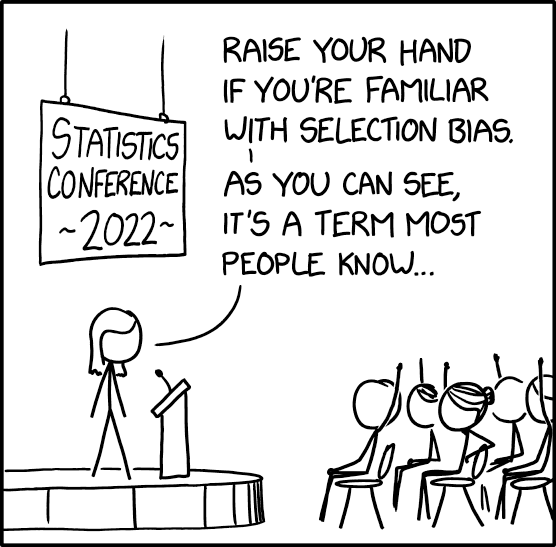
\includegraphics[width = 0.45\linewidth]{selection_bias_xkcd.png}
\end{center}
\end{frame}


\begin{frame}{¿Por qué responder estás preguntas es difícil? (Parte II)}
\begin{wideitemize}
	\item
	Responder preguntas causales es incluso \textit{más difícil} que las descriptivas. ¿Por qué?
	
	\pause
	\item
	Las preg. causales envuelven tanto un componente descriptivo (¿cómo es el \textit{outcome} en la realidad?) y un componente \textbf{contrafactual} (¿cómo hubieran sido las cosas bajo un tratamiento diferente?)
	
	\pause
	\item
	Ejemplo: ¿Cuál es el efecto causal en sus salarios de ir a UdeP en vez de la U. Pacífico?
		\begin{itemize}
			\item
			Preg. Descriptiva: ¿Cuánto ganan los alumnos de UdeP después de graduarse?
			
			\item
			Preg. Contrafactual: ¿Cuánto \textit{hubieran} ganado los alumnos de UdeP después de graduarse \textit{si hubieran estudiado en la UP}?
		\end{itemize}
		
	\pause 	
	\item Preg. Contrafactuales no se pueden contestar con data solamente. ¡Necesitamos supuestos para aprender de ellos!
	
\end{wideitemize}	
\end{frame}



\begin{frame}{Partir el problema}
	\begin{wideitemize}
		
		\item
		Al pensar en preg. causales, suele ser mejor partir el problem en dos
		
		\item
		\textbf{Identificación:} ¿qué podemos aprender de los parámetros que nos importan (efectos causales) si tuvieramos \textit{data observable} de toda la población

		\begin{itemize}
			\item 
			Necesitamos hacer supuestos sobre cómo los outcomes observados se relacionan con los outcomes que hubieran sucedido bajo distinto tratamiento
			
		\end{itemize}
		
		\item
		\textbf{Estadística}: ¿qué podemos aprender sobre la población desde la muestra finita que tenemos en la práctica?
			\begin{itemize}
				\item 
				Necesitamos entender el proceso de cómo se genero la data para la población completa
			\end{itemize} 	
		
	\end{wideitemize}	
	
\end{frame}



\begin{frame}{Mapa conceptual para entender estos pasos}
	
\begin{wideitemize}

\item \textbf{Muestra:} la data observable
	\begin{itemize}
		\item
		Encuesta a alumnos graduados de UdeP y UP sobre sus salarios
	\end{itemize}

\pause
\item \textbf{Estimador:} una función de la data en la muestra
	\begin{itemize}
		\item Diferencia en salario promedio entre UdeP y UP en la encuesta
	\end{itemize}

\pause
\item \textbf{Estimando:} función de la data de la \textit{población}
	\begin{itemize}
		\item Diferencia en la \textit{media} salarial entre UdeP y UP
	\end{itemize}

\pause 
\item \textbf{Parámetro (estructural) objetivo:} lo que realmente nos importa conocer
	\begin{itemize}
		\item Efecto causal de ir a UdeP relativo a UP en salarios
	\end{itemize}

\end{wideitemize}	

\medskip
\pause
\begin{wideitemize}

\item El proceso para ir al \textit{estimando} desde el \text{estimador} construido con tu \textit{muestra} se llama \textbf{estimación/inferencia estadística}.

\pause 
\item El proceso para aprender del \textit{parámetro} desde el \textit{estimando} es llamado \textbf{identificación}.

\end{wideitemize}
	
\end{frame}





\begin{frame}
\vspace{-10mm}
	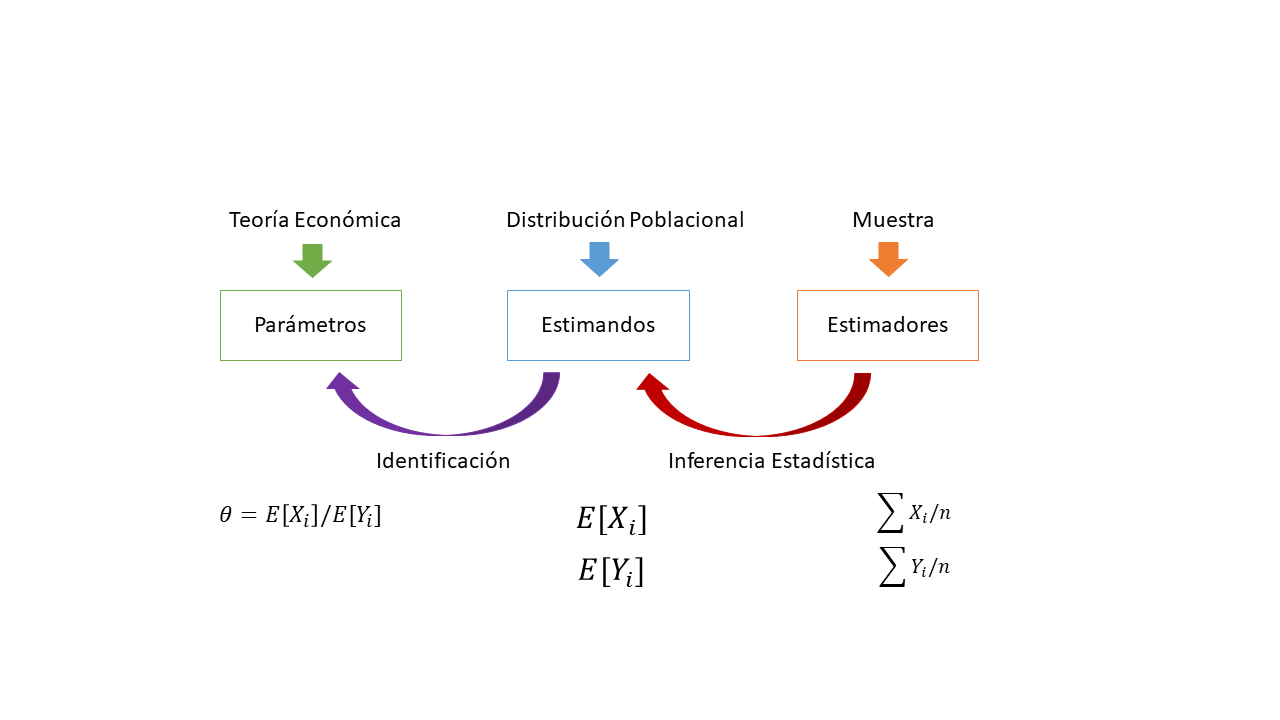
\includegraphics[width=1.2\textwidth]{BigPicture}
\end{frame}


\begin{frame}{Agreguemosle un poquito de mate...}
\begin{wideitemize}
	\item Introduciremos la notación de \textbf{potential outcomes} 
		\begin{itemize}
			\item 
			¡Conceptualmente es muy útil para pensar acerca de causalidad! 
		\end{itemize}
	
	\pause 
	\item $D_i$ = indicator si recibo el tratamiento (1 si UdeP, 0 si UP)
	
	\pause
	\item $Y_i(1)$ = outcome si tratado = salarios de UdeP
	\item $Y_i(0)$ = outcome si control = salarios de UP
	
	\pause 
	\item El outcome observado $Y_i$ es $Y_i(1)$ si $D_i = 1$ y $Y_i(0)$ si $D_i = 0$. ($Y_i$ es tu salario \textit{actual})
	
	\pause
	\item
	Podemos reescribir el outcome observado como $Y_i = D_i Y_i(1) + (1-D_i) Y_i(0)$
\end{wideitemize}

\end{frame}



\begin{frame}
\begin{wideitemizeshort}
	\item
	Ejemplo de muestra: $(Y_i,D_i)$ para $i=1,...N$. Data de salarios y donde fuiste a la universidad
	
	\pause 
	
	\item
	Ejemplo de estimador: 
		\begin{itemize}
			\item
			Diferencia en la media muestral de salarios de gente que fue a UdeP, y de gente que fue a UP
			
			$$ \underbrace{\frac{1}{N_1} \sum_{i:D_i=1} Y_i}_{\text{Salario prom de UdeP}} - \underbrace{\frac{1}{N_0} \sum_{i:D_i=0} Y_i}_{\text{Salario prom de UP}}$$		
		\end{itemize}
	
	\pause
		\item
		Ejemplo estimando: 	
		
				\begin{itemize}
			\item
			Diferencia en media poblacional salarial entre gente que fue UdeP y UP 
			
			$$\underbrace{ E[ Y_i | D_i = 1] }_{\text{Media salarial de UdeP}} - \underbrace{E[Y_i | D_i = 0]}_{\text{Media salarial de UP}}$$
		 
		\end{itemize}
	\pause 
	
	\item
	Ejemplo parámetro objetivo:
		\begin{itemize}
			\item Efecto causal de ir a UdeP en salarios:
			$\underbrace{E[Y_i(1) | D_i =1]}_{\text{Salarios de UdeP para gente de UdeP en la pob.}} - \underbrace{E[Y_i(0) | D_i = 1]}_{\text{Salarios de UP para gente de UdeP en la pob.}} $.   
		\end{itemize}
\end{wideitemizeshort}
\end{frame}


\begin{frame}{¿Por qué es difícil la identificación causal?}
	
	\begin{wideitemize}
		
		\item
		Experimento mental: imagina que tenemos data de salarios para \textit{todos} los graduados de UdeP y UP		
		
		\item
		Podemos aprender esto de la data:
		$$\color{teal} \underbrace{E[ Y_i(1) | D_i=1  ] }_{\text{Salarios de UdeP para alumnos UdeP}} \hspace{0.5cm}  \text{and} \hspace{0.5cm} \underbrace{E[Y_i(0) | D_i = 0]	}_{\text{Salarios de UP para alumnos UP}}$$
		
		\pause 
		\item
		El efecto causal de ir a UdeP dentro de los graduados UdeP es 
		$$ \color{teal}{\underbrace{E[ Y_i(1) | D_i=1  ] }_{\text{Salario de UdeP para alumnos UdeP}}} - \color{red}{ \underbrace{E[ Y_i(0) | D_i=1  ] }_{\text{Salarios de UP para alumnos UdeP}}}$$ 
		
		\pause 
		\item
		La data no me dice $\color{red}{ \underbrace{E[ Y_i(0) | D_i=1 ] }_{\text{Salarios de UP para alumnos UdeP}}}$. ¿Por qué no? 
		\pause
			\begin{itemize}
				\item 
				¡Porque jamás podremos ver la vida de los alumnos de UdeP si hubieran hipotéticamente ido a UP!
			\end{itemize} 
		
	\end{wideitemize}
	
\end{frame}


\begin{frame}
	\begin{wideitemize}
		\item
		Una idea para arreglar este problema es asumir que: 
		
		$$ \color{red}{ \underbrace{E[ Y_i(0) | D_i=1  ] }_{\text{Salarios de UP para alumnos UdeP}}} = \color{teal}{ \underbrace{E[ Y_i(0) | D_i=0 ] }_{\text{Salarios de UP para alumnos UP}}}$$
		
		\item
		¿Por qué esto puede darnos la respuesta incorrecta? 
		
		\pause
		
		\item
		Porque los alumnos UdeP pueden ser diferentes de los alumnos UP en muchas maneras que afectarian sus salarios (irrespectivamente de a cual de las dos universidades fueron)
		
			\begin{itemize}
				\item 
				Habilidad académica, entorno e ingresos familiares, metas laborales, etc.
			\end{itemize}
		
		\item
		Estas diferencias se les llaman \textit{variables omitidas} o, en inglés, \textit{confounding factors}
	\end{wideitemize}
\end{frame}

\begin{frame}{Experimentos}
\begin{wideitemize}
\item
El estándar de oro para aprender sobre causalidad son los llamados  \textit{randomized controlled trial (RCT)}, aka experimentos

\item
Imaginen que podemos aleatorizar quienes van a que universidad (asumamos que solo existen UdeP y UP por simplicidad)

\item
Como la universidad es aleatoriamente asignada, lo único distinto entre la gente de UdeP y UP es la universidad a la que atendieron

\item
Por tanto, 

		$$ \color{red}{ \underbrace{E[ Y_i(0) | D_i=1  ] }_{\text{Salarios de UP para alumnos UdeP}}} = \color{teal}{ \underbrace{E[ Y_i(0) | D_i=0 ] }_{\text{Salarios de UP para alumnos UP}}}$$
		
		dado que eliminamos los \textit{confounding factors}


\end{wideitemize}
\end{frame}

\begin{frame}{Pero correr experimentos suele ser difícil/imposible}
	\begin{wideitemize}
	
	\item
	Desgraciadamente, por temas de ética no podemos aleatorizar quién va a qué universidad

	\item
	De la misma manera, no puedes convencer al gobierno de que aleatorice donde subir el salario mínimo, u otras políticas
	
	\item
En pocas palabras, aleatorizar no solo es difícil sino que puede ser inmoral dado que hablamos de sujetos humanos
	
		\begin{itemize}
			\item 
			``¿Cuál es el efecto causal de que fallezca algún familiar?''
		\end{itemize}	
	
	\pause
	\item
	Un gran componente de su rama de econometría trata sobre herramientas que podemos usar los economistas cuando los experimentos no son posibles
	\end{wideitemize}
\end{frame}

\begin{frame}{Hacia esto vamos\dots}
	\begin{wideitemize}
		\item
		\textbf{Revisión de probabilidad/estadística}. Para tener un mismo lenguaje matemático para poder discutir
		
			\begin{enumerate}
				\item 
				\textit{Estimación/Inferencia Estadística: }como la muestra se relaciona con la población de interés
				
				\item
				\textit{Identification:} como las características observables de la población se relacionan a parámetros (causales) que nos importan
			\end{enumerate}
		\pause 
		
		\item
		\textbf{Regresión lineal y predicción: }Discutiremos el método de mínimos cuadrados (en inglés, Ordinarly Least Squares, OLS), la forma de estimación más utilizada por economistas. ¿Cuándo funciona y cuándo falla?
		
		\pause
		\item
		\textbf{Regularización: }Discutiremos brevemente el método LASSO para lidiar con el caso en que hacemos una predicción utilizando muchísimas características (\textit{alta dimensionalidad})
			 
	\end{wideitemize}
\end{frame}

	
	%%%%%%%%%%% Prob/stats 
	
	\begin{frame}{Outline}
	
	1. Media Condicional
	\vspace{0.8cm}
	
	
	2. Muestreo Aleatorio
	
	\vspace{0.8cm}
	3. Test de Hipótesis e Inferencia
	
		\vspace{0.8cm}
	4. Teoría Asintótica	
\end{frame}


\begin{frame}{Variable aleatoria y CDF}
\begin{wideitemize}
\item
Una \textbf{variable aleatoria} es un resumen numérico de un proceso aleatorio (formalmente, es una función de los elementos del espacio muestral)

\begin{itemize}
\item Por ej. $X$ es el número de ``caras'' que vemos al tirar una moneda 10 veces; $X=1$ si llueve, 0 de lo contrario. 
\end{itemize}
\pause{}

\item Una variable aleatoria real se caracteriza por su \textbf{distribución de función acumulada} (CDF), 

$$F(x) = Pr( X \leq x ) $$

\noindent que dice la probabilidad de que $X$ tome el valor $x$ o algun valor menor
\medskip\pause{}
\begin{itemize}
\item Nota: minusculas ``$x$'' suele denotar realizaciones (es decir, números no aleatorios) de variables aleatorias como ``$X$'' ...
\end{itemize}

\end{wideitemize}
\end{frame} 	
	
	

\begin{frame}{Esperanza Condicional}
\vspace{0.2cm}
En economía nos interesa conocer la \textbf{esperanza condicional}

\begin{itemize}
\item ¿Cuál es el promedio $Y$ cuando $X=x$ (por ej. cual es mi salario si mi universidad fue UdeP)?
\pause 
	
\item La función de esperanza condicional (CEF): \\$E[Y\mid X=x]=\sum_{y\in\mathbb{Y}} y p(y\mid x)$ si es discreta \\
$E[Y\mid X=x]=\int_{y\in\mathbb{Y}} y f(y\mid x) dy$ si es continua

\vspace{0.1cm}\pause{}
\item A veces se escribe $E[Y\mid X]$ para el CEF \uline{aleatorio} evaluado en $X$ (var. aleatoria)
\vspace{0.1cm}\pause{}
\item Decimos que $Y$ es \emph{independiente en media} de $X$ cuando $E[Y\mid X=x]=E[Y]$ para todo $x$
\vspace{0.1cm}\pause{}
\item Condicionar en $X$ hace que sea una función constante: por ej. $E[f(X)+g(X)Y|X=x]=f(x)+g(x)E[Y|X=x]$ para cualquier $f(\cdot)$, $g(\cdot)$
\end{itemize}

\end{frame}


\begin{frame}{Esperanza Condicional}
	\vspace{0.2cm}
	CEF del (logaritmo) del ingreso anual dado años de educación
	
	\begin{center}
		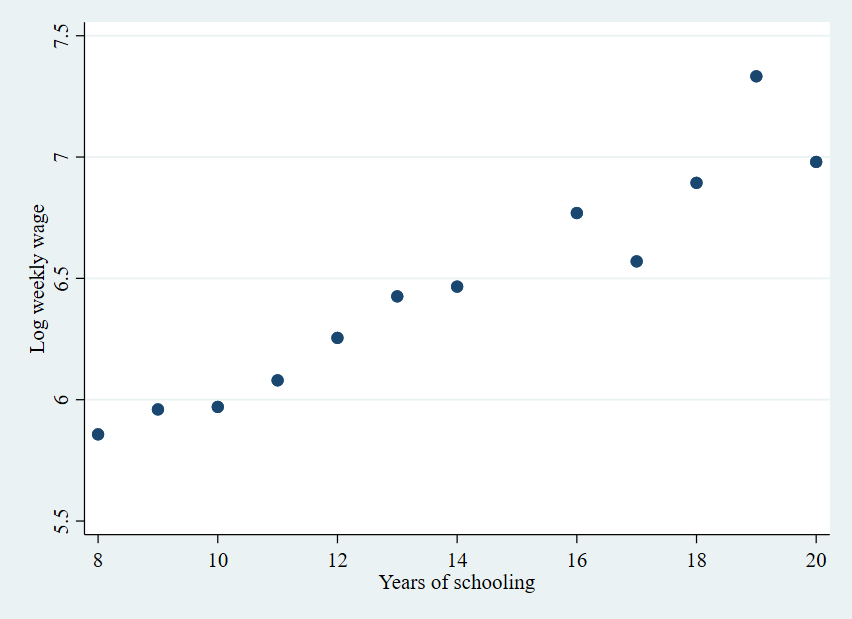
\includegraphics[scale=1.3]{stata2pre.png}
	\end{center}
	
\end{frame}

\begin{frame}{Ley de Esperanzas Iteradas (LIE)}
Uno de los resultados más importantes que usamos es está ley llamada en inglés \textbf{Law of Iterated Expectations} (LIE)
\vspace{0.2cm}

Veamos un ejemplo. Supongamos que queremos calcular la altura promedio de personas en Perú. Entonces la LIE dice que podemos:
\vspace{0.2cm}

1) Calcular el promedio de altura en hombres. \\ \vspace{0.2cm}

2) Calcular el promedio de altura en mujeres. \\ \vspace{0.2cm}

3) Calcular un promedio ponderado entre la altura hombres y mujeres (proporcional a la fracción de personas que son mujeres)

\vspace{0.2cm}
\pause
Matemáticamente estamos diciendo lo siguiente

\begin{align*}
E[altura] &= P(mujer) E[altura | mujer] + P(hombre) E[altura|hombre] \\ \pause{}
& =  E[ E[altura | sexo ]  ]	
\end{align*}
 



\end{frame}


\begin{frame}{Ley de Esperanzas Iteradas (LIE)}
	La versión formal de la \textbf{Ley de Esperanzas Iteradas} (LIE) es:
	\begin{align*}
		E[Y]=E[E[Y\mid X]]\pause{}
	\end{align*}
	Note que la esperanza de la izquierda usa la distribución de $Y$ ($p(y)$); la esperanza de la parte fuera de la derecha usa $p(x)$, mientras que la esperanza interna usa la distribución condicional $p(y\mid x)$
	
\end{frame}



\begin{frame}{Independencia en Media vs No Correlacionado}
\vspace{0.2cm}
LIE muestra que independencia en media ($E[Y\mid X]=E[Y]$) implica que las variables no están correlacionadas

\begin{align*}
Corr(X,Y)&\propto E[(X-E[X])(Y-E[Y])]\\ \pause{}
&=E[E[(X-E[X])(Y-E[Y])\mid X]]\\ \pause{}
&= E[(X-E[X])E[Y-E[Y]\mid X]]\\\pause{}
&= E[(X-E[X])(E[Y\mid X]-E[Y])]\\\pause{}
&= 0\text{, when $E[Y\mid X]=E[Y]$}
\end{align*}
\vspace{0.3cm}
¡Asegúrense de entender cada paso!
\vspace{0.5cm}

El converso de esta proposición no es cierto: estar no correlacionado no implica que sean independientes en media

\begin{itemize}
\item Por supuesto, independencia $\implies$ independencia en media (pero no a la otra dirección $\impliedby$)
\end{itemize}

\end{frame}
	
\begin{frame}{Outline}
	
	\textcolor{red!75!green!50!blue!25!gray}{1. Media Condicional} $\checkmark$
	\vspace{0.8cm}
	
	
	2. Muestreo Aleatorio
	
	\vspace{0.8cm}
	3. Test de Hipótesis e Inferencia
	
	\vspace{0.8cm}
	4. Teoría Asintótica		
\end{frame}


\begin{frame}{Defiendo una muestra}
	\begin{wideitemize}	
	
	\item
	Para formalizar el trabajo de la inferencia estadística debemos especificar cómo la data observada se saca de la población	
	
	\pause{}
	

	\item Baseline: observamos una muestra \textit{representativa} de tamaño N que es \emph{independente e idénticamente distribuida} (\emph{iid}) por ej. $\mathbf{Y}=[Y_{1},Y_{2},\dots,Y_{N}]^\prime$
	
	\pause{}\smallskip
\begin{itemize}
	\item \emph{Independiente}: $Y_i$ es independiente de $Y_j$ para todo $i\neq j$
	
\smallskip
	\pause{}
	\item \emph{Idénticamente Distribuido}: $Y_i$ y $Y_j$ tienen la misma distribución para todo $i,j$

\pause{}
\smallskip
	\item
	\emph{Representativo:} La distribución de $Y_i$ es la misma que la distribución de la población de interés
	
\end{itemize}		
	\pause	
	\item	
	Data \emph{iid} y representativa es un caso base que es relativamente fácil de analizar, pero es importante saber que no necesariamente se cumple en la práctica
		\begin{itemize}
			\pause
\smallskip
			\item
			si muestreamos gente dentro de un mismo hogar, esas observaciones no son independientes 
		
\smallskip	
			\pause
			\item
			si muestreamos de manera estratificada dentro de cada departamento, no es identicamente distribuido
			\pause

\smallskip
			\item 
			En el ejemplo de Dewey v. Truman no era representativo! 
		\end{itemize}
	\end{wideitemize}

\end{frame}



\begin{frame}{Media y Varianza de Promedio Muestral}
\vspace{0.1cm}
Suponga que queremos saber sobre la media poblacional $\mu=E[Y_i]$ de una muestra representativa \emph{iid} $\mathbf{Y}$ de tamaño $N$\pause{} 
\pause{}
\begin{itemize}
\item Un estimador natural es el \emph{promedio muestral}: $\hat{\mu}=\frac{1}{N}\sum_i Y_{i}$
\vspace{0.1cm}\pause{}
\item $\hat{\mu}$ es una función de la data aleatoria $\mathbf{Y}$. Por lo tanto es una variable aleatoria, tiene una distribución (también llamada ``distribución muestral'')
\end{itemize}
\vspace{0.2cm}
\pause{}

Calculemos la media y varianza de $\hat{\mu}$
\begin{align*}
E[\hat{\mu}]&=E\left[\frac{1}{N}\sum_i Y_i\right]=\pause\frac{1}{N}\sum_i E[Y_i]=\pause\mu\\\pause{}
Var(\hat{\mu})&=Var\left(\frac{1}{N}\sum_i Y_i\right)=\pause{}\frac{1}{N^2}\sum_iVar(Y_i)=\pause{}\sigma^2/N,
\end{align*}
donde $\sigma^2=Var(Y_i)$ 
\pause{}

\begin{itemize}
\item Ecuación (1) dice que $\hat{\mu}$ es \emph{insesgado}: su media es $\mu$
\vspace{0.1cm}
\pause{}
\item Ecuación (2) dice que la desviación estándar de $\hat{\mu}$ desde su media $\mu$ se achica a medida que $N$ crece ($\approx$ \emph{consistencia})
\end{itemize}

\end{frame}

\begin{frame}{Muestreo Aleatorio y Promedio Muestral}
\vspace{0.2cm}
Simulen insesgadez  y consistencia para estimar la media de ingresos:

\begin{center}
\includegraphics[scale=0.45]{stata18.png} \includegraphics[scale=0.5]{stata19.png}
\end{center}

\end{frame}

\begin{frame}{Simulations of Random Sampling}
\vspace{0.2cm}
Simulen insesgadez  y consistencia para estimar la media de ingresos:

\begin{center}
\includegraphics[scale=0.45]{stata18.png} \includegraphics[scale=0.5]{stata20.png}
\end{center}

\end{frame}

\begin{frame}{Random Sampling and Sample Means}
\vspace{0.2cm}
Simulen insesgadez  y consistencia para estimar la media de ingresos:

\begin{center}
\includegraphics[scale=0.45]{stata18.png} \includegraphics[scale=0.5]{stata21.png}
\end{center}

\end{frame}

\begin{frame}{Muestreo Aleatorio y Promedio Muestral}
\vspace{0.2cm}
Simulen insesgadez  y consistencia para estimar la media de ingresos:

\begin{center}
\includegraphics[scale=0.45]{stata18.png} \includegraphics[scale=0.5]{stata22.png}
\end{center}

\end{frame}

\begin{frame}{Muestreo Aleatorio y Promedio Muestral}
\vspace{0.2cm}
Simulen insesgadez  y consistencia para estimar la media de ingresos:

\begin{center}
\includegraphics[scale=0.45]{stata18b.png} \includegraphics[scale=0.5]{stata23.png}
\end{center}

\end{frame}

\begin{frame}{Muestreo Aleatorio y Promedio Muestral}
\vspace{0.2cm}
Entonces, dos razones por las que $\hat{\mu}=\frac{1}{N}\sum_i Y_i$ es un buen estimador de $\mu=E[Y_i]$:

\begin{itemize}
\item Es insesgado: $E[\hat{\mu}]=\mu$
\vspace{0.1cm}
\item Su varianza se encoge a 0 a medida que la muestra crece: $\lim_{N\rightarrow\infty}Var(\hat{\mu})=0$ 
\end{itemize}
\vspace{0.5cm}


\end{frame}


%\begin{frame}{Random Sampling and Sample Means V}
%\vspace{0.2cm}
%\uline{Fun with Notation}: we can write this CEF estimator as 
%\begin{align*}
%\hat{\mu}(x)=\frac{1}{N_x}\sum_{i:X_i=x}Y_i=\frac{\sum_{i}D_{ix}Y_i}{\sum_{i}D_{ix}}
%\end{align*}
%where $D_{ix}=\mathbf{1}[X_i=x]$ is an indicator for $X_i$ taking on value $x$ (why?)
%\vspace{0.4cm}
%\pause{}
%
%In vector form, we can write this as
%\begin{align*}
%\hat{\mu}(x)=(\mathbf{D_x}^\prime \mathbf{D_x})^{-1} \mathbf{D_{x}}^\prime \mathbf{Y}
%\end{align*}
%for $\mathbf{D_x}=[D_{x1},\dots,D_{xN}]^\prime$
%
%\pause{}
%\vspace{0.4cm}
%
%Furthermore if we collect $\mathbf{D}=[\mathbf{D_{x_1}},\mathbf{D_{x_2}},\dots,\mathbf{D_{x_K}}]$, then we can write the vector of CEF estimates $\hat{\boldsymbol\mu}=[\hat{\mu}(x_1),\hat{\mu}(x_2),\dots,\hat{\mu}(x_K)]^\prime$ as 
%\begin{align*}
%\hat{\boldsymbol\mu}=(\mathbf{D}^\prime \mathbf{D})^{-1} \mathbf{D}^\prime \mathbf{Y}
%\end{align*}\pause{}
%\vspace{-0.5cm}
%
%\begin{itemize}
%\item This shows $\hat{\boldsymbol\mu}$ is an ordinary least squares (OLS) linear regression estimator, which you'll learn to love soon...
%\end{itemize}
%
%\end{frame}

\begin{frame}{Outline}
	
	\textcolor{red!75!green!50!blue!25!gray}{1. Media Condicional} $\checkmark$
	\vspace{0.8cm}
	
	
	\textcolor{red!75!green!50!blue!25!gray}{2. Muestreo Aleatorio} $\checkmark$
	
	\vspace{0.8cm}
	3. Test de Hipótesis e Inferencia
	
	\vspace{0.8cm}
	4. Teoría Asintótica	
	
\end{frame}

\begin{frame}{Test de Hipótesis - Intro}
\begin{wideitemize}

\item
Vimos que cuando $N$ es largo, el promedio $\hat\mu$ se acerca mucho a la media $\mu$

\item
¿Pero qué significa estar ``cerca''?

\item
Si el promedio es \$50,000, ¿es razonable pensar que la media verdara puede ser \$55,000? ¿Y qué tal \$70,000? 

\pause
\item
\textbf{Test de hipótesis} nos ayuda a formalizar el concepto de ``cercanía''.

\pause
\item
Nos dice que tan probable es ver un promedio muestral de \$50,000 si la media verdadera es \$55,000,  \$70,000, etc.

\end{wideitemize}
\end{frame}


\begin{frame}{Overview de Test de Hipótesis}

\begin{enumerate}
	\item 
	Especificamos la \textbf{hipótesis nula} que la media poblacional toma cierto valor, $H_0: \mu = \mu_0$.
\smallskip
		\begin{itemize}
			\item 
			Por ej. La media poblacional es \$55,000 significaria que $H_0: \mu = 55,000$
			\end{itemize}
	
	\medskip
	\pause
	\item
	Calculamos que tan probable es observar $\hat\mu$ por lo menos tan lejos como observamos de $\mu_0$ si la nula es verdad. Esto se llama un \textbf{$\mathbf{p}$-value}
	\medskip
	\pause
	\item
	\textbf{Rechazamos} si el $p$-value es pequeño, i.e.: es poco probable que observemos un $\hat\mu$ tan lejano de $\mu_0$ si la nula fuera cierta
\smallskip
		\begin{itemize}
		\pause 
		\item
		El umbral más común es $\alpha=0.05$ 
	\end{itemize}
	
	\vspace{.1cm}
	\pause
	\item
	
	Podemos construir un \textbf{intervalo de confianza} (CI) que colecciona todos los posibles valores de $\mu_0$ que \textit{no podemos rechazar} de esta manera
		\begin{itemize}
			\pause
			\item
			El CI, por construcción, contiene el verdadero valor $\mu$ en 95\% de las realizaciones de la data cuando $\alpha = 0.05$ 
		\end{itemize}
\end{enumerate}
	
\end{frame}


\begin{frame}{Test de Hipótesis con $\hat\mu$ Normalmente Distribuido }
\begin{itemize}
	\item 
	Trabajemos sobre este caso especial en todos sus pasos: $\hat\mu \sim \mathrm{N}(\mu, \sigma^2/N)$ con $\sigma^2$ known. 
	\medskip
	\pause
	\item
	¿Por qué considerar este caso?
\smallskip
		\begin{itemize}
			\item 
			$\mathrm{N}(\mu, \sigma^2/N)$ es la exacta distribución de $\hat\mu$ si $Y_i \overset{iid}{\sim} \mathrm{N}(\mu,\sigma^2)$ \pause
			\smallskip
			\item
			En un rato mostraremos que incluso si $Y_i$ no es normal, $\hat\mu$ es aprox. normal para $N$ grande
\smallskip\pause{}
\item También mostraremos que con $N$ grande podemos estimar $\sigma^2$ arbitrariamente bien
		\end{itemize}

	\pause
	\item
	Suponga que queremos testear $H_0:\mu=\mu_0$ (por ej. media de ingresos es \$55,000)
	
	
	\item
	Definimos $\hat{t} = \dfrac{\hat\mu - \mu_0 }{ \sigma /\sqrt{N} }$, y note que bajo la nula $\hat{t} \sim \mathrm{N}(0,1)$ 
	\begin{itemize}
	\pause
	\item
	La distribución de $\hat{t}$ es sobre muestras repetidas provenientes de la muestra  $(Y_1,...,Y_N)$.
		\end{itemize}
\end{itemize}
\end{frame}

\begin{frame}{Test de Hipótesis con $\hat\mu$ Normalmente Distribuido (cont.) }
\begin{wideitemize}
\item
Bajo la nula, $H_0:\mu=\mu_0$, $\hat{t} \sim \mathrm{N}(0,1)$.

\pause
\item ¿Qué es $Pr( |\hat{t}| > t )$ para algún $t \geq 0$? \pause
$$ Pr( |\hat{t}| > t ) = 1 - Pr(|\hat{t}| \leq t) \pause = 1 - Pr(  -t \leq \hat{t} \leq t  ) = \pause 1 - (\Phi(t) - \Phi(-t))$$ 
\vspace{-0.8cm}
\item
Definimos el $p$-value para la nula como $H_0: \mu = \mu_0$ as 
\begin{align*}
 p(\hat{t}) = 1 - (\Phi( |\hat{t} | ) - \Phi(- |\hat{t} |  )  ) \pause{} &= 1-  \left(  \Phi \left(  \frac{|\hat\mu - \mu_0|}{\sigma / \sqrt{N}} \right)  -  \Phi \left(  \frac{-|\hat\mu - \mu_0|}{\sigma / \sqrt{N}} \right) \right) 	\\
 &\pause{}= 2\left(1 -  \Phi \left(  \frac{|\hat\mu - \mu_0|}{\sigma / \sqrt{N}} \right)  \right) 
\end{align*}

 
\item
Intuitivamente, $p$ es la probabilidad de observar un $|\hat{t}|$ por lo menos así de grande si la nula es verdadera

\end{wideitemize}	
\end{frame}

\begin{frame}{Ilustración de Construcción de P-Value}
	
	
	\begin{center}
		Standard Normal PDF (mean zero, unit std. dev.)
		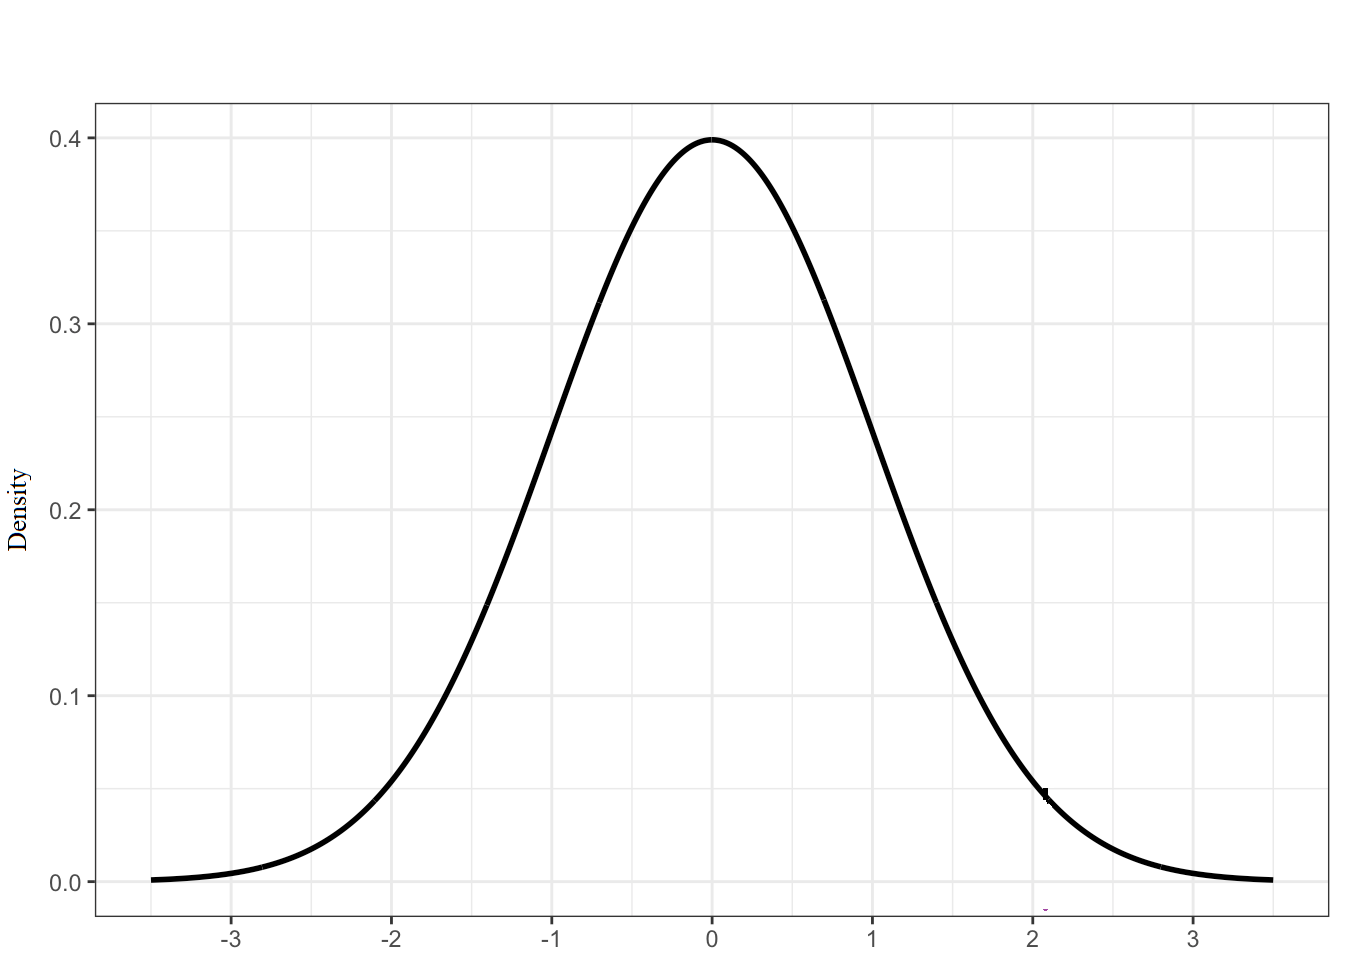
\includegraphics[scale=0.3]{pvalue1.png}
	\end{center}
	
\end{frame}

\begin{frame}{Ilustración de Construcción de P-Value}
	
	
	\begin{center}
		Normalized realization of the random estimator
		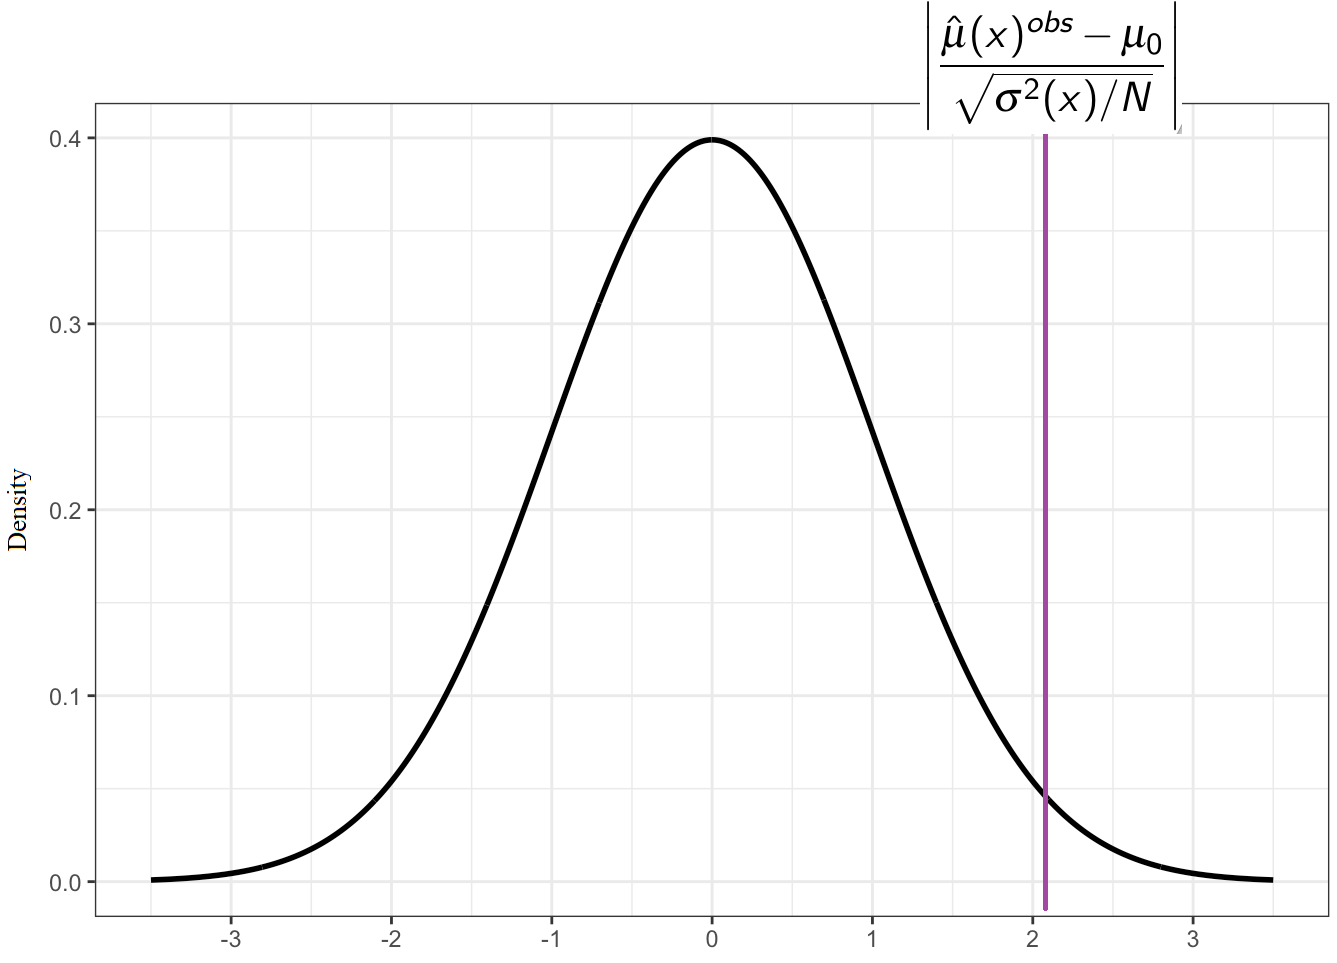
\includegraphics[scale=0.3]{pvalue2.png}
	\end{center}
	
\end{frame}

\begin{frame}{Illustration of P-Value Construction}		
	\begin{center}
		p-value calculation
		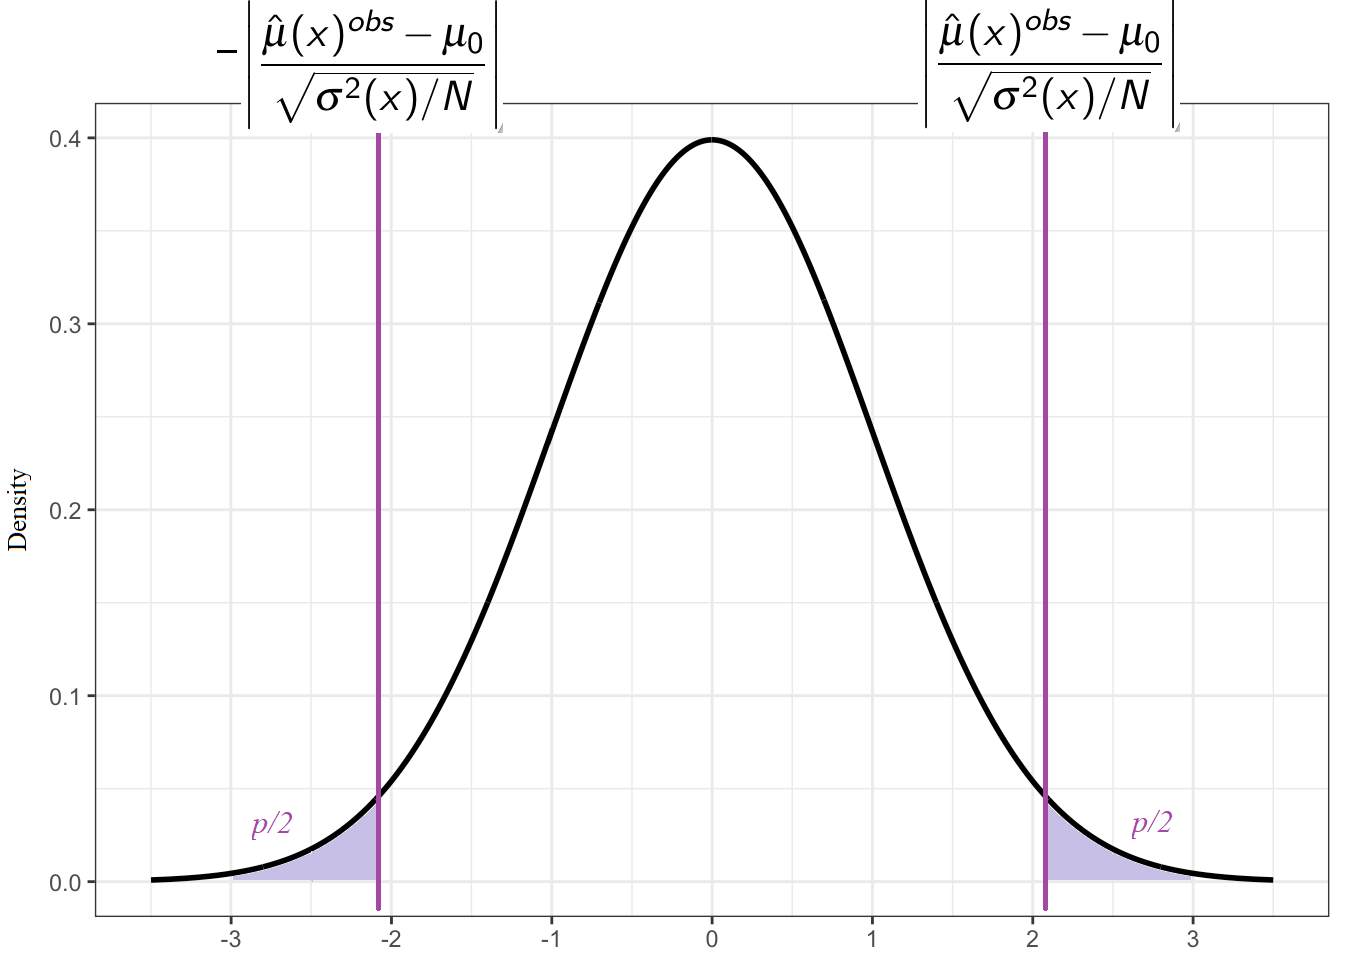
\includegraphics[scale=0.3]{pvalue3.png}
	\end{center}
\end{frame}




\begin{frame}{¿Cuándo rechazar la nula?}

\begin{wideitemize}
	\item 
	Recuerden que el $p$-value toma la forma
	$$1 - \left(  \Phi(|\hat{t}|) - \Phi( -|\hat{t}| )  \right) $$
	
	\item
	Resulta que $\Phi(1.96) - \Phi(-1.96) \approx 0.95$. Entonces, $p < 0.05$ si y solo sí $|\hat{t}| > 1.96$. Por lo tanto rechazamos al nivel de  5\% si $|\hat{t}| > 1.96$. 
	
	\pause
	\item
	¿Qué implica esto sobre el valor de $\mu_0$ que rechazamos/no rechazamos?
	
	\pause
	\item
	No rechazamos si 	
	$$ |\hat{t}| \leq 1.96 \pause \implies \dfrac{ |\hat\mu - \mu_0| }{ \sigma / \sqrt{N} } \leq 1.96 \pause \implies \mu_0 \in  [\hat\mu - 1.96 \sigma / \sqrt{N} , \hat\mu + 1.96 \sigma \sqrt{N}]$$
\vspace{-0.5cm}
	\pause
	\item
	El intervalo $\hat\mu \pm 1.96 \sigma / \sqrt{N}$ es por tanto el 95\% intervalo de confianza (CI)
	\smallskip

		\begin{itemize}
			\item 
			Tiene la propiedad de que $Pr( \mu_0 \in CI ) = 0.95$ cuando $H_0: \mu = \mu_0$ es verdadero
		\end{itemize}
	
\end{wideitemize}
	
\end{frame}



\begin{frame}{Dos Formas de Fregarla}
	
	\begin{center}
	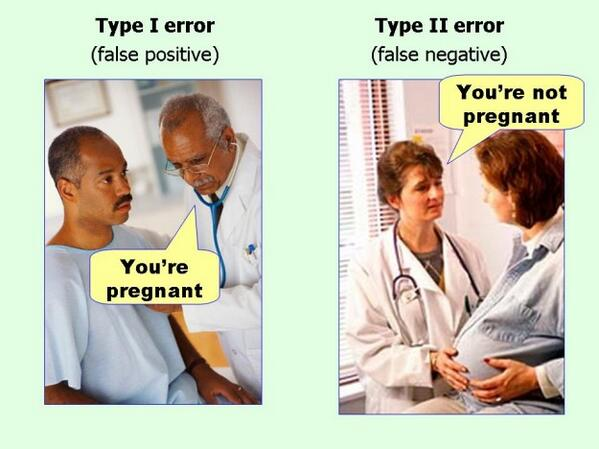
\includegraphics[scale=0.5]{type_errors.jpg}
	\end{center}

\end{frame}


\begin{frame}{Significancia y Poder Estadístico}
	
	\begin{itemize}
		\item El \emph{nivel de significancia} (suele decirsele solo \emph{size}) de un test es la probabilidad pre-especificada de incorrectamente rechazar la nula cuando es verdad ( \% error tipo I)
		 \pause
		 \begin{itemize}
		 	\item 
		 	Por ej. un test al 5\% rechaza cuando $p<0.05$.
		 \end{itemize}
		\pause
		\bigskip

		\item El \emph{poder} de un test es la probabilidad de correctamente rechazar la nula cuando es falsa (1- \% error tipo II)
		
			\begin{itemize}
				\item 
				El poder es una función de la hipótesis \textit{alternative}. 
				\item 
				Ejemplo 1:la probabilidad de rechazar $H_0:\mu=\mu_0$ cuando en realidad $\mu = \mu_A$
				\item 
				Ejemplo 2: es más probable rechazar que yo soy Brad Pitt a que soy Pedro Castillo (mayor poder)
			\end{itemize}
	\end{itemize}

\end{frame}




\begin{frame}{Precaución sobre interpretar $P$-Value }

\begin{itemize}
\item A veces los p-values se interpretan como la ``probabilidad de que $H_0$ es verdad.'' ¿Es esto correcto? \pause{} ¡No!


\begin{wideitemize}
	\item $p$-value dice la probabilidad de obtener la data observada \emph{asumiendo} que la nula es verdad
	
	\item Es decir, $p$-value nos dice sobre $P(data | H_0)$, no $P(H_0 | data)$. 

	\item Por la regla de Bayes, $P(H_0 | Data) = P(Data | H_0) * P(H_0) / P(Data)$. Para formalizar esto, debemos tomar una postura sobre cual es nuestra creencia previa sobre si $H_0$ es verdadera, $P(H_0)$.
	
\end{wideitemize}


\pause
\bigskip
\item La gente interpreta $p<0.05$ como fuerte evidencia de que hay un efecto, y $p \geq 0.05$ como evidencia de no efecto. 

	\begin{itemize}
		\item 
		Pero $p=0.05$ es un umbral arbitrario. 
		\vspace{0.1cm}
		\item
		Mejor vean el $p$-value como un espectro indicando que tan probable es que veamos la data observada dada la hip. nula.
 \pause
		\vspace{0.1cm}
		\item
		Además, $p$-values pueden ser super altos cuando la nula es verdadera (¡bajo poder estadístico!)
	\end{itemize}
\end{itemize}

\end{frame}



\begin{frame}{¿Qué hacemos con data no-normal?}
\vspace{0.2cm}
\begin{itemize}
\item Ok, chévere ... ¿y ahora que hacemos con la data de la vida real?
\pause{}
\smallskip

\begin{itemize}
\item ¡Casi todas las variables no tienen esta distribución!\pause{}
\vspace{0.1cm}
\item ¡¿Incluso si fueran normales, cómo saber su varianza verdadera?!\pause{}
\vspace{0.1cm}
\item ¡¿Les acabo de hacer perder un buen par de horas!?! \pause{} No \dots espero :) \pause{}
\end{itemize}
\vspace{0.4cm}

\item Ahora veremos que pasa en el mundo de las muestras grandes: \textbf{asymptopia}. Esto nos permitirá aplicar inferencia similar incluso cuando la muestra $Y_i$ no sea normalmente distribuida.
\end{itemize}

\end{frame}

%%%%%%%%%% Asymptotics 




\begin{frame}{Outline}
	
	\textcolor{red!75!green!50!blue!25!gray}{1. Media Condicional} $\checkmark$
	\vspace{0.8cm}
	
	
	\textcolor{red!75!green!50!blue!25!gray}{2. Muestreo Aleatorio} $\checkmark$
	
	\vspace{0.8cm}
	\textcolor{red!75!green!50!blue!25!gray}{3. Test de Hipótesis e Inferencia} $\checkmark$
	
	\vspace{0.8cm}
	4. Teoría Asintótica	
	
\end{frame}

\begin{frame}{Motivación}

\begin{wideitemize}
	
\item 
Hemos visto el caso de hacer test de hipótesis sobre media poblacional usando $\hat\mu$ cuando es \textbf{normalmente distruibida} con una varianza conocida

\item
Esto surge del caso en que $Y_i\sim \mathrm{N}(\mu,\sigma^2)$ caundo $\sigma$	es conocido

\item
Esta situación es bastante rara\dots ¿cómo hacemos inferencia de manera general?

\pause

\item
Afortunadamente, el supuesto de que el promedio muestral está normalmente distribuido resulta ser una buena \textbf{aproximación} cuando la muestra es grande

\pause
\item
A lo que nos referimos con  ``buena aproximación'' es algo formalizado por la teoría asintótica, que considera la distribución de $\hat\mu$ en el límite cuando $N \rightarrow \infty$
	
\end{wideitemize}		

\end{frame}


\begin{frame}{Resumen de Resultados Importantes}
	
\begin{wideitemize}

\item La \textbf{Ley de los Grandes Números} (LLN) dice que cuando $N$ es grande, $\hat\mu$ está cerca de $\mu$ con probabilidad muy alta


\pause
\item El \textbf{Teorema del Límite Central} (CLT) dice que cuando $N$ es grande, la distribución de $\hat\mu$ es aproximadamente normal con media $\mu$ y varianza $\sigma^2/n$

\pause
\item El \textbf{Continuous Mapping Theorem} dice que cuando $N$ es grande, las funciones continuas de $\hat\mu$, digamos $g(\hat\mu)$, también son cercanas a $g(\mu)$


\end{wideitemize}	
\end{frame}




\begin{frame}{Convergencia en Probabilidad}
	
\begin{wideitemize}
\item
Intuitivamente, una variable aleatoria $X_N$ \textbf{converge en probabilidad} a $x$ si la probabilidad de que $X_N$ está ``cerca'' a $x$ es casi 1 cuando $N$ es grande

\pause
\item
Formalmente, decimos que $X_N$ converge en probabilidad a $x$,  $X_n \rightarrow_p x$, si para todos los $\epsilon > 0$,

$$\lim_{N\rightarrow \infty}P(|X_N - x| > \epsilon) \rightarrow 0 $$

\pause
\item 
Si $X_n \rightarrow_p x$ para una constante $x$, decimos que $X_n$ es \textit{consistente} para $x$

	
\end{wideitemize}

\end{frame}


\begin{frame}{Convergencia en Probabilidad (Cont.)}
	
\begin{wideitemize}

\item Hecho útil: si $E[ (X_N - x)^2 ] \rightarrow 0$, entonces $X_N \rightarrow_p x$

\pause

\item 
\textbf{Prueba} (recuerden que en este curso no se les pedirá derivar estas cosas): \\

Por ley de esperanzas iteradas (LIE),
\begin{align*}
E[ (X_N - x)^2 ]=& P( |X_n - x| > \epsilon ) E[ (X_N - x)^2 | |X_n - x| > \epsilon ] + \\
& P( |X_n - x| \leq \epsilon ) E[ (X_N - x)^2 | |X_n - x| \leq \epsilon ]	 \\
\pause \geq &  P( |X_n - x| > \epsilon ) \epsilon^2 + 0 
\end{align*}
\pause
\noindent  Esto implica que 
$$P( |X_N - x|  > \epsilon ) \leq E[ (X_N - x)^2  ] / \epsilon^2 \text{ (Chebychev's Inequality)  }$$
\pause 
Por tanto, $E[ (X_N - x)^2  ] \rightarrow 0$ implica $P( |X_N - x|  > \epsilon ) \rightarrow 0$

\end{wideitemize}	
\end{frame}


\begin{frame}{Ley de los Grandes Números}
	
\begin{wideitemize}
	
\item \textbf{Ley de los Grandes Números}. Suponga que $Y_1,...,Y_N$ son sacados $iid$ de una distribución con $Var(Y_i) = \sigma^2 < \infty$. Entonces $$\hat\mu_N = \frac{1}{N} \sum_{i=1}^{N} Y_i \rightarrow_p \mu = E[Y_i]$$

\item
En cristiano: si la muestra se hace grande, la media muestral se volverá cercana a la media poblacional con alta probabilidad.

\pause
\item
\textbf{Prueba:} Como saben $E[\hat\mu_N] = \mu$ y $Var(\hat\mu_N) = \sigma^2 / N$.  \\

Entonces, $$Var(\hat\mu_N) = E[ (\hat\mu_N - \mu )^2 ] = \sigma^2/N \rightarrow 0 $$ \\

Por tanto, $\hat\mu_N \rightarrow_p \mu$ por nuestro ``hecho útil''. 
\end{wideitemize}	
	
\end{frame}



\begin{frame}{Ilustración de LLN}
	\vspace{0.2cm}
	Distribución y media de $\frac{1}{N}\sum_i Z_i$ cuando $Z_i\sim \mathrm{U}(0,1)$, $\mathbf{N=1}$
	
	\begin{center}
		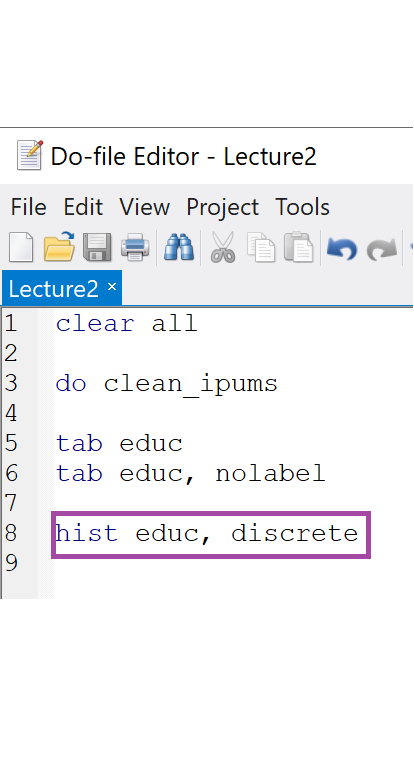
\includegraphics[scale=0.4]{Stata5.png} 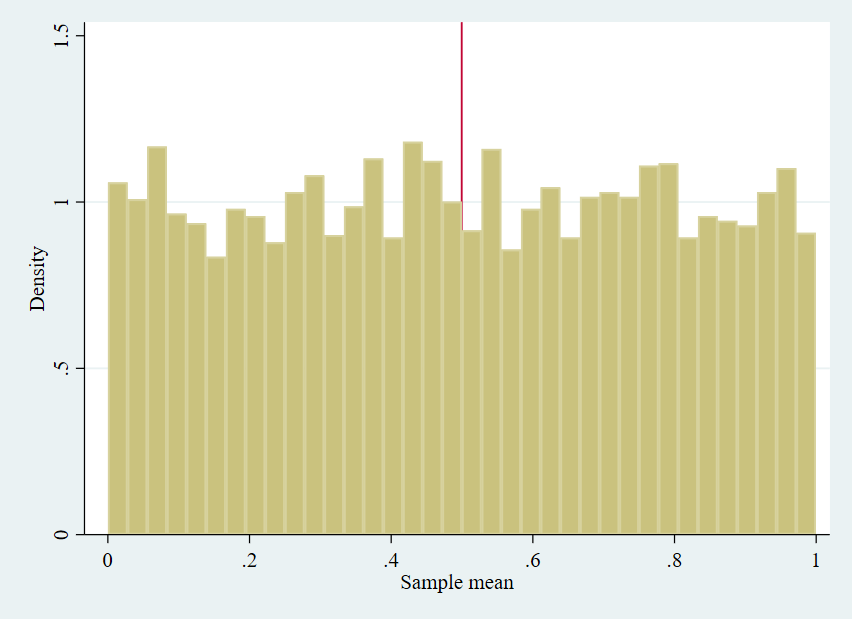
\includegraphics[scale=0.25]{sims1_2.png}
	\end{center}
	
\end{frame}

\begin{frame}{Ilustración de LLN}
	\vspace{0.2cm}
	Distribución y media de $\frac{1}{N}\sum_i Z_i$ cuando $Z_i\sim \mathrm{U}(0,1)$, $\mathbf{N=10}$
	
	\begin{center}
		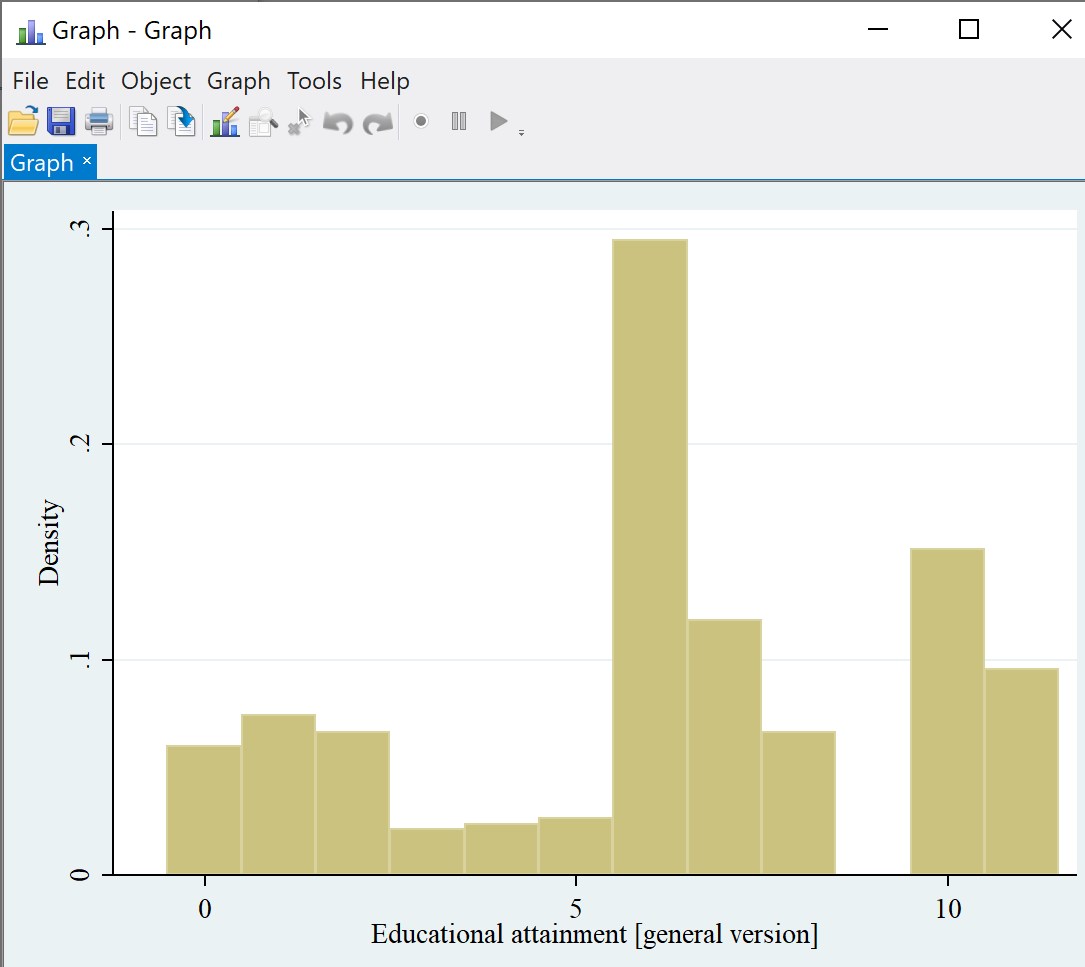
\includegraphics[scale=0.4]{Stata6.png} 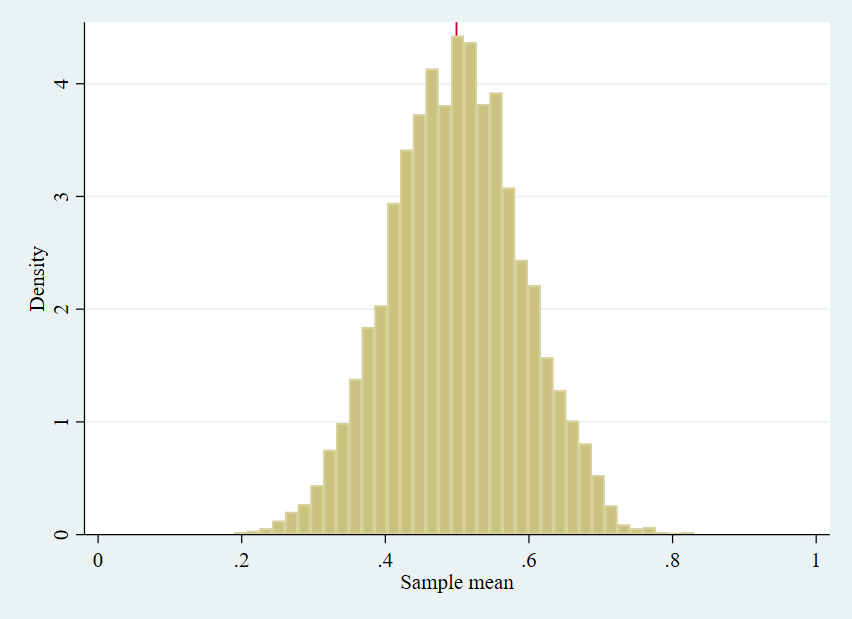
\includegraphics[scale=0.25]{sims10_2.png}
	\end{center}
	
\end{frame}

\begin{frame}{Ilustración de LLN}
	\vspace{0.2cm}
	Distribución y media de $\frac{1}{N}\sum_i Z_i$ cuando $Z_i\sim \mathrm{U}(0,1)$, $\mathbf{N=100}$
	
	\begin{center}
		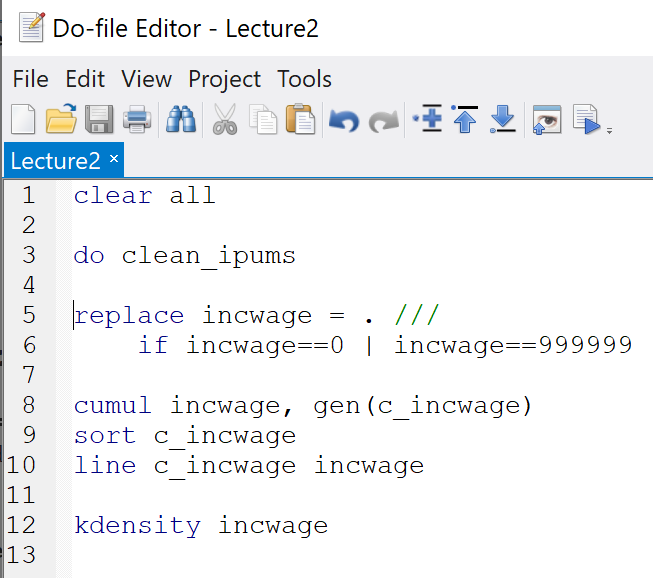
\includegraphics[scale=0.4]{Stata7.png} 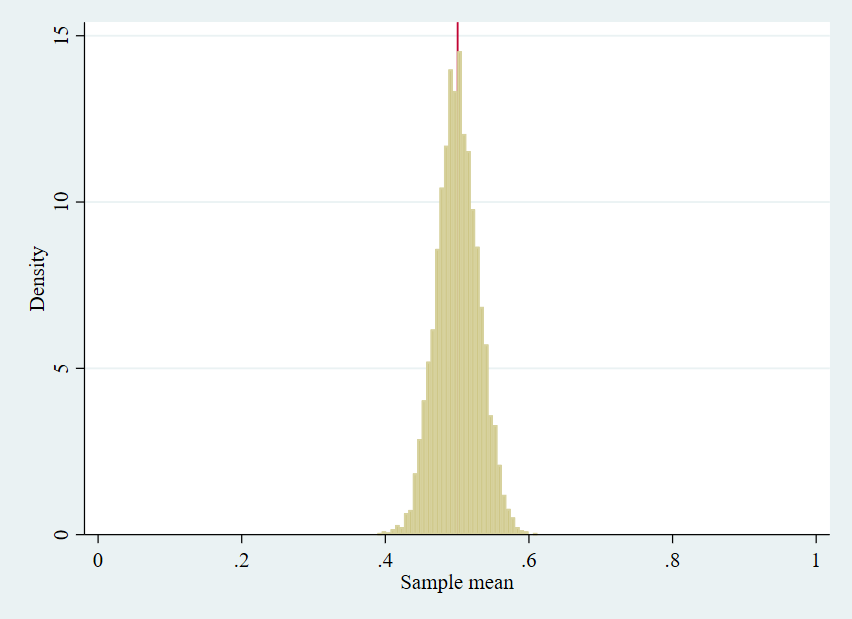
\includegraphics[scale=0.25]{sims100_2.png}
	\end{center}
	
\end{frame}

\begin{frame}{Laws of Large Numbers Illustration}
	\vspace{0.2cm}
	Distribution and mean of $\frac{1}{N}\sum_i Z_i$ when $Z_i\sim \mathrm{U}(0,1)$, $\mathbf{N=1000}$
	
	\begin{center}
		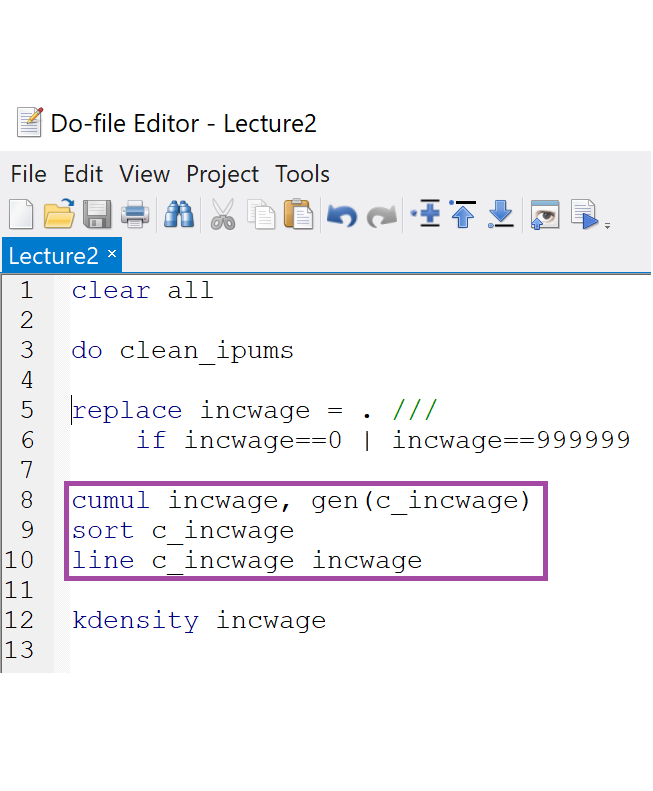
\includegraphics[scale=0.4]{Stata8.png} 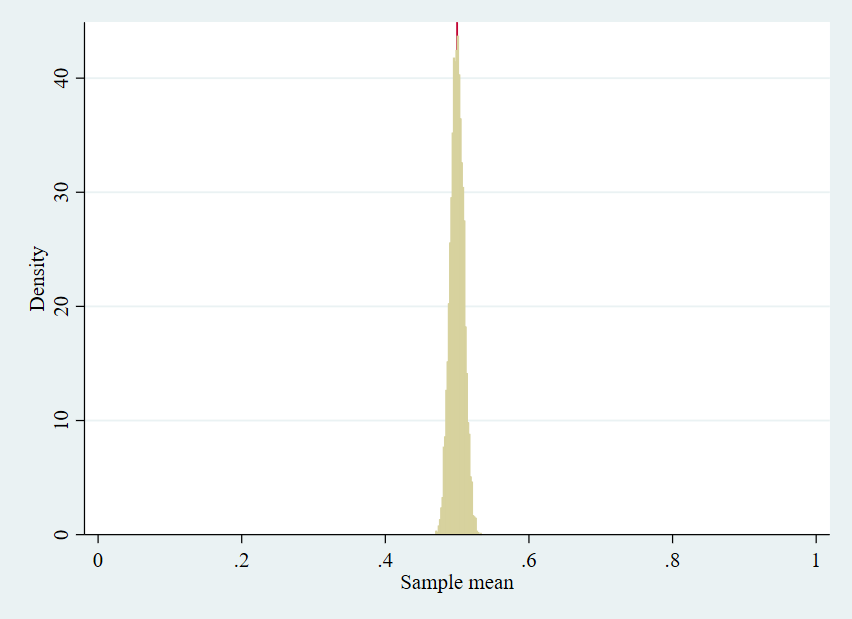
\includegraphics[scale=0.25]{sims1000_2.png}
	\end{center}
	
\end{frame}


\begin{frame}{Convergencia en Distribución}
	
	\begin{wideitemize}

		\item
		Se habrán dado cuenta que la distribución de $\hat\mu$ en la simulación se aproxima a una normal cuando $N$ se vuelve grande
		
		\item
		La noción de \textbf{convergencia en distribución} formaliza lo que significa que dos distribuciones se aproximen  entre ellas		
		
		\pause
		\item
		Definición: Decimos que $X_N$ converge en distribución a una variable continuamente distribuida $X$, denotado por $X_n \rightarrow_d X$ o $X_n \Rightarrow X$, si el CDF de $X_N$ converge (punto por punto - pointwise) al CDF de $X$,
		
		$$F_{X_N}(x) \rightarrow F_{X}(x) \text{ para cada punto } x$$ 
		
		
%		\pause
%		\item
%		\emph{Technical note}: if the limit $X$ is discrete, we only require $F_{X_N}(x) \rightarrow F_{X}(x)$ at points where $F(x)$ is continuous
%		
%			\begin{itemize}
%				\item
%				For example, if $X_N = 1/N$ and $X = 0$, then we say $X_N \rightarrow_d X$ even though $F_{X_N}(0) = 0$ for all $N$ while $F_X(0) = 1$
%			\end{itemize}
	\end{wideitemize}
	
\end{frame}


\begin{frame}{Teorema del Límite Central}
\begin{wideitemize}

\item
\textbf{The Central Limit Theorem (CLT)} formalizes the sense in which sample means are approximately normally distributed in large samples

\pause
\item
Theorem: Suppose that $Y_1,...,Y_N$ are drawn $iid$ from a distribution with mean $\mu = E[Y_i]$ and variance $Var(Y_i) = \sigma^2 < \infty$. Then the sample mean $\hat\mu = \frac{1}{N} \sum_{i=1}^N Y_i$ satisfies

$$ \sqrt{N} (\hat\mu - \mu) \rightarrow_d N(0, \sigma^2) $$


\pause
\item
In words, the theorem says the following: 


\begin{enumerate}
\normalsize{
\item 
We can start with any distribution $Y_i$, possibly non-normal 

\item
If we take the average of the $Y_1,...,Y_N$ in a sample sufficiently large, the distribution of $\hat\mu = \frac{1}{N} \sum_i Y_i$ is (approximately) normal! 
}
\end{enumerate}

\end{wideitemize}	

\end{frame}



\begin{frame}{Ilustración de CLT}
	\vspace{0.2cm}
	Distributions of $\hat{\mu}=\frac{1}{N}\sum_i X_i$ vs. $\mathrm{N}(E[\hat\mu],Var(\hat{\mu}))$: $X_i\sim \mathrm{U}(0,1)$, $\mathbf{N=1}$
	
	\begin{center}
		
\includegraphics[scale=0.4]{Stata1.png} 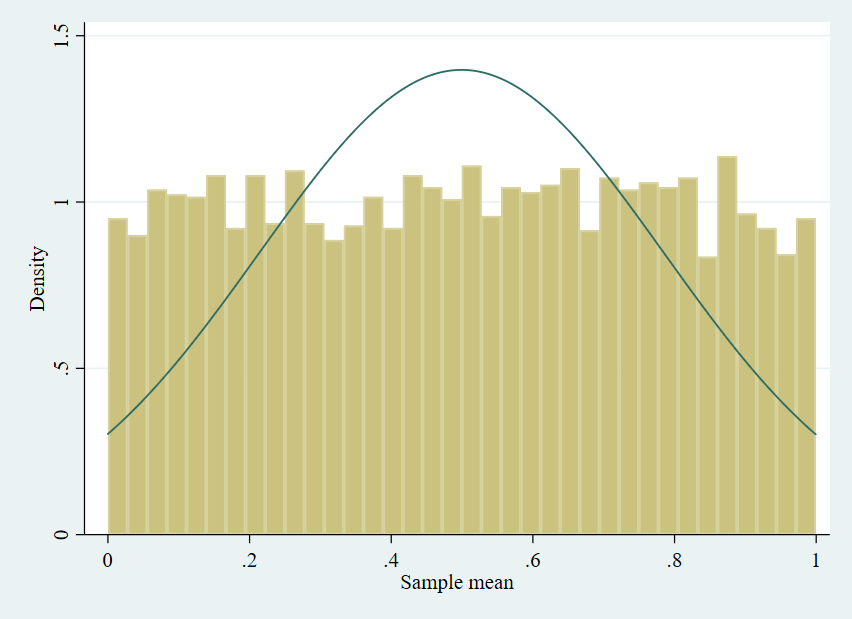
\includegraphics[scale=0.25]{sims1.png}
	\end{center}
	
\end{frame}

\begin{frame}{Ilustración de CLT}
	\vspace{0.2cm}
	Distributions of $\hat{\mu}=\frac{1}{N}\sum_i X_i$ vs. $\mathrm{N}(E[\hat\mu],Var(\hat{\mu}))$: $X_i\sim \mathrm{U}(0,1)$, $\mathbf{N=2}$
	
	\begin{center}
		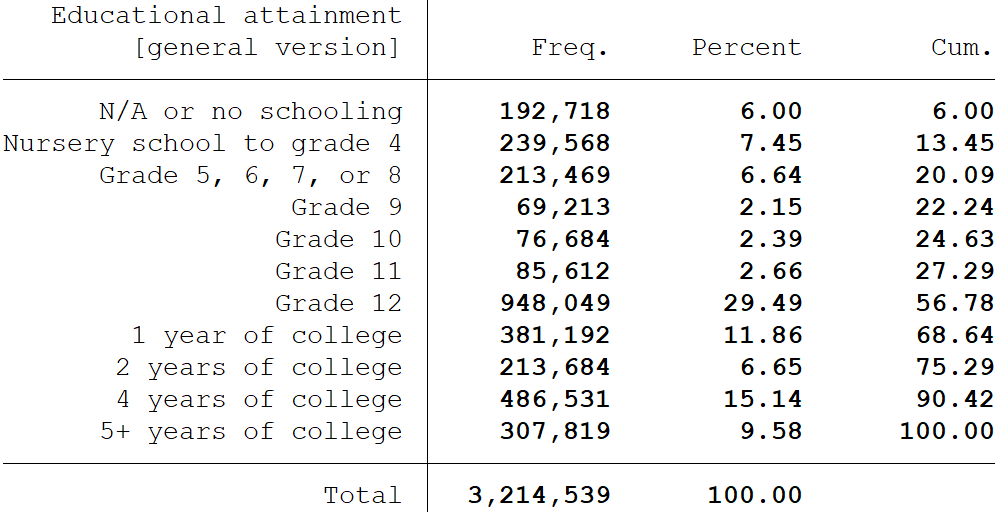
\includegraphics[scale=0.4]{Stata2.png} 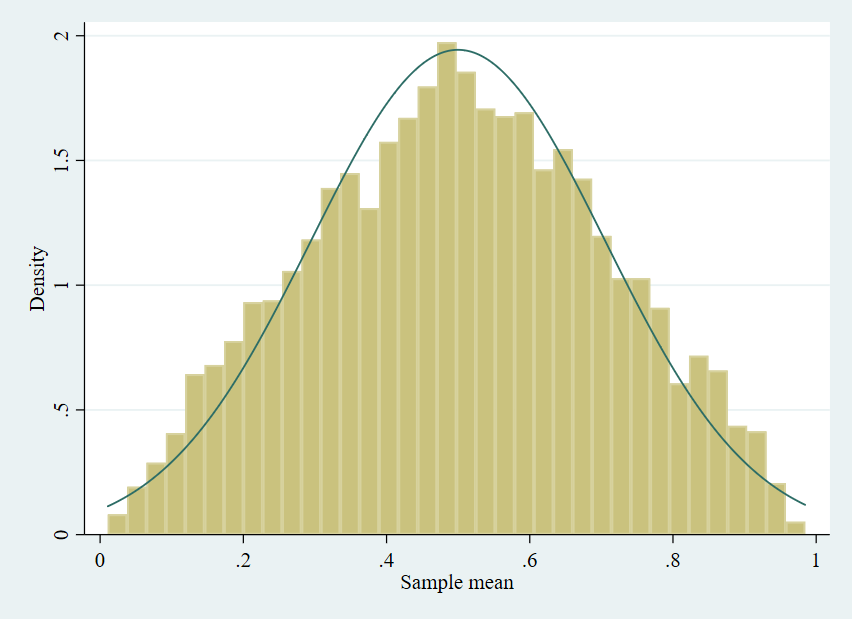
\includegraphics[scale=0.25]{sims2.png}
	\end{center}
	
\end{frame}

\begin{frame}{Ilustración de CLT}
	\vspace{0.2cm}
	Distributions of $\hat{\mu}=\frac{1}{N}\sum_i X_i$ vs. $\mathrm{N}(E[\hat\mu],Var(\hat{\mu}))$: $X_i\sim \mathrm{U}(0,1)$, $\mathbf{N=5}$
	
	\begin{center}
		
\includegraphics[scale=0.4]{Stata3.png} 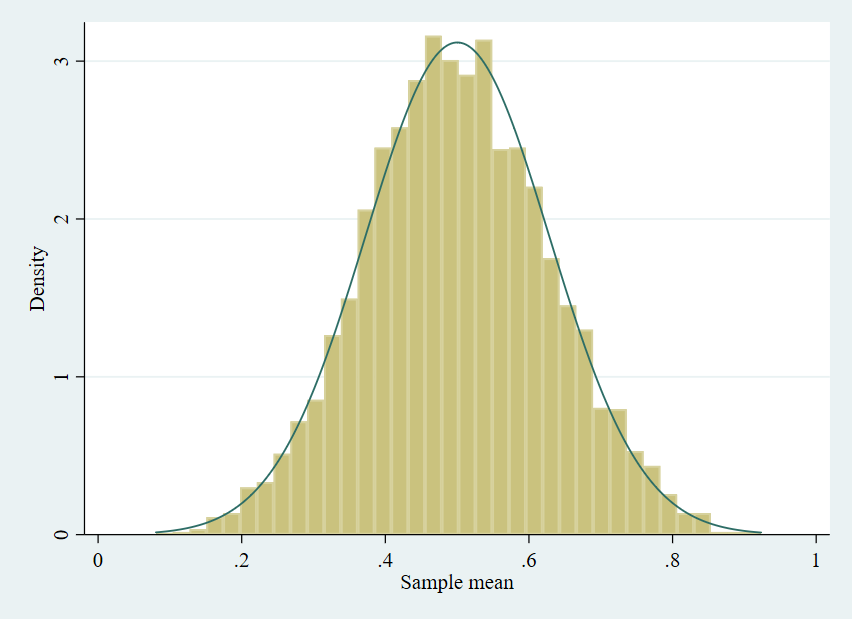
\includegraphics[scale=0.25]{sims5.png}
	\end{center}
	
\end{frame}

\begin{frame}{Ilustración de CLT}
	\vspace{0.2cm}
	Distributions of $\hat{\mu}=\frac{1}{N}\sum_i X_i$ vs. $\mathrm{N}(E[\hat\mu],Var(\hat{\mu}))$: $X_i\sim \mathrm{U}(0,1)$, $\mathbf{N=10}$
	
	\begin{center}
		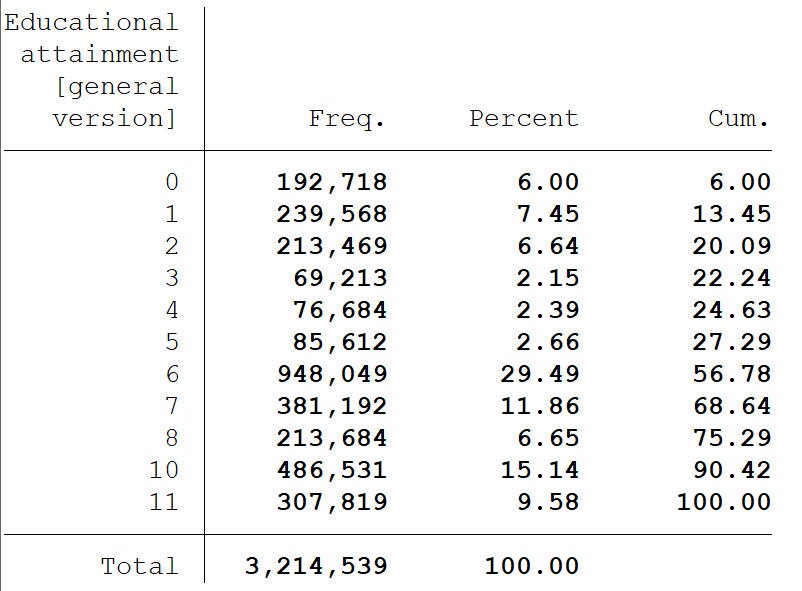
\includegraphics[scale=0.4]{Stata4.png} 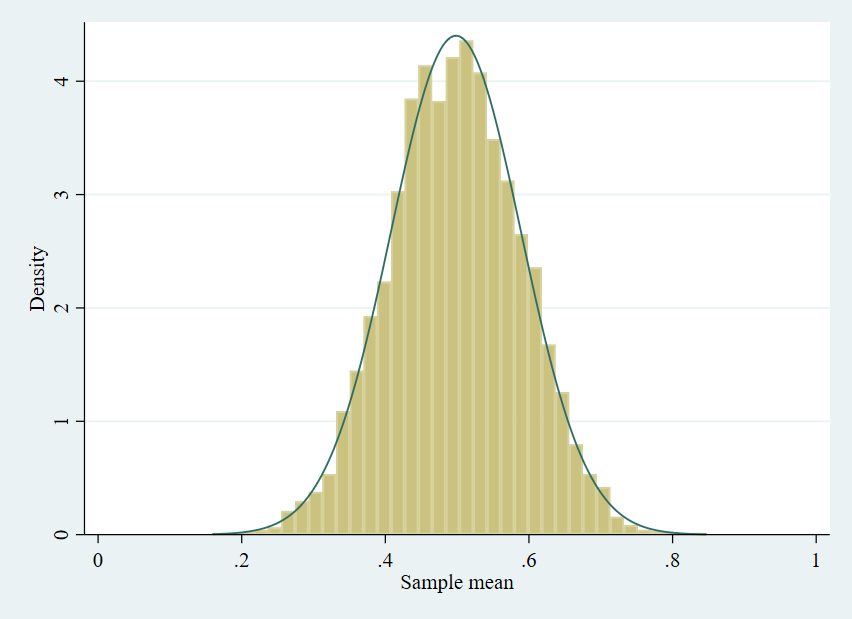
\includegraphics[scale=0.25]{sims10.png}
	\end{center}
	
\end{frame}


\begin{frame}{No puede ser :o }
	\centering
	
\includegraphics[width = 0.5\linewidth]{surprise.jpg}
\end{frame}




\begin{frame}{Continuous Mapping Theorem}

\begin{wideitemize}	

\item
A veces estamos interesado en funciones de la media muestral (por ej., el estadístico $t$ es una función de $\hat\mu$ and $\sigma$).

\pause
\item
El \textbf{continuous mapping theorem} (CMT) nos dice que pasa con funciones continuas de variables aleatorias que convergen en distribución/probabilidad

\pause
\item
Teorema: supongamos que $g(\cdot)$ es una función continua\\
\vspace{.2cm}

Si $X_N \rightarrow_p X$, entonces $g(X_N) \rightarrow_p g(X)$ \\
\vspace{.2cm}
\pause

Si $X_N \rightarrow_d X$, entonces $g(X_N) \rightarrow_d g(X)$\\
\vspace{0.2cm}
\pause{}

En el caso multivariado es igual: Si $\mathbf{X_N} \rightarrow_p \mathbf{X}$, then $g(\mathbf{X_N}) \rightarrow_p g(\mathbf{X})$ y si $\mathbf{X_N} \rightarrow_d \mathbf{X}$, entonces $g(\mathbf{X_N}) \rightarrow_d g(\mathbf{X})$

\end{wideitemize}

\end{frame}


\begin{frame}{Convergencia de Varianza Muestral}
\begin{wideitemize}
\item
Una apllicación util del CMT es probar la convergencia en probabilidad de la varianza muestral

\pause
\item
Escribimos  $\hat\sigma^2 = \frac{1}{N} \sum_{i=1}^N (Y_i - \hat\mu)^2$ como la varianza muestral de $Y_i$.

\pause
\item
Claim: si $Y_1,...,Y_N$ son $iid$ y $Var(Y_i^2)$ es finito, entonces $\hat\sigma^2 \rightarrow_p \sigma^2 = Var(Y_i)$. 

\pause
\item
Prueba: \\

Podemos escribir la varianza muestral como $\hat\sigma^2 = \frac{1}{N} \sum_{i=1}^N Y_i^2 - \hat\mu^2$. \\ \vspace{.1cm} \pause

Primer término: por LLN, $ \frac{1}{N} \sum_{i=1}^N Y_i^2 \rightarrow_p E[Y_i^2]$. \\ \vspace{.1cm} \pause

Segundo término: por LLN, $\hat\mu \rightarrow_p \mu = E[Y_i]$. Entonces, por el CMT, $\hat\mu^2 \rightarrow_p E[Y_i]^2$.\\ \vspace{.1cm} \pause

Aplicando nuevamente el CMT, $\frac{1}{N} \sum_{i=1}^N Y_i^2 - \hat\mu^2 \rightarrow_p E[Y_i^2] - E[Y_i]^2 = \sigma^2$. 

\end{wideitemize}		
\end{frame}

\begin{frame}{Lemma de Slutsky}

\begin{wideitemize}

\item
\textbf{Lemma de Slutsky} (a veces también llamado Teorema) resume \textit{casos especiales} del CMT que son útiles

\pause
\item
Supongamos que  $X_N \rightarrow_p c$ para una constante $c$, y $Y_N \rightarrow_d Y$. Entonces: 

\item
$X_N + Y_N \rightarrow_d c + Y$. \pause

\item
$X_n Y_n \rightarrow_d c Y$. \pause

\item
If $c \neq 0$, then $Y_n/ X_n \rightarrow_d Y /c$. 

\pause
\item
Versiones análogas a esto aplican para vectores de variables aleatorias.
\end{wideitemize}
	
\end{frame}

\begin{frame}{Test de Hipótesis Asintótico}

\begin{wideitemize}
\item
Recuerden que cuando $Y_i \sim \mathrm{N}(\mu,\sigma^2)$, mostramos que el $t$-statistic $\hat{t} = \frac{\hat\mu - \mu_0}{\sigma / \sqrt{n}} \sim  \mathrm{N}(0,1)$ bajo $H_0: \mu = \mu_0$.

\pause
\item 
Entonces, cuando $Y_i \sim \mathrm{N}(\mu,\sigma^2)$, teniamos que $Pr(|\hat t| > 1.96) = 0.05$ bajo la nula.

\pause
\item
Ahora, suponemos que $Y_i$ no es normalmente distribuida y no sabemos su varianza.

\pause
\item
Por CLT, $\sqrt{N} (\hat\mu - \mu_0) \rightarrow_d N(0,\sigma^2)$.\\
Por CMT y LLN (como se mostró arriba), $\hat\sigma \rightarrow_p \sigma$. 

\pause
\item
Entonces, por Slutsky's, $\hat{t} = \dfrac{\hat\mu - \mu_0}{ \hat\sigma /\sqrt{n} } \rightarrow_d N(0,1)$.

\pause
\item
Por tanto, asintóticamente $Pr( |\hat{t}| > 1.96 ) \rightarrow 0.05$, incluso cuando $Y_i$  no es normal y $\hat\sigma$ is estimado! Podemos hacer test de hipótesis igual que antes.

\end{wideitemize}	
	
\end{frame}


\begin{frame}{Test de Hipótesis Asintótico}

\begin{wideitemize}
\item
Similarmente, cuando $Y_i$ era normal con $\sigma$ conocido, mostramos que el intervalo de confianza $\hat\mu \pm 1.96 \sigma/\sqrt{N}$ contiene el verdadero $\mu$ 95\% de las veces (asumiendo como cierta la nula)

\pause
\item
De manera análoga, cuando $Y_i$ es no-normal con varianza desconocida, $\hat\mu \pm 1.96 \hat\sigma/\sqrt{N}$ contiene el verdadero $\mu$ con probabilidad aproximando 95\% a medida que $N$ se vuelve grande.

\end{wideitemize}
	
\end{frame}

\begin{frame}{Example -- Oregon Health Insurance Experiment}
	
\begin{center}
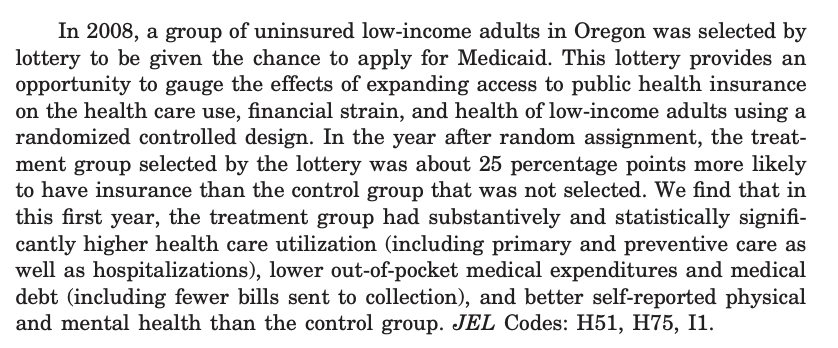
\includegraphics[width = 0.9 \linewidth]{ohie-abstract}	
\end{center}
\end{frame}


\begin{frame}{Ejemplo: acceso a salud y depresión}

\begin{tabular}{lll}
 & Grupo Control & Grupo Tratamiento \\
 Media & 0.329 & 0.306\\
 DesvEst & 0.470 &  0.461 \\
 N & 10426 & 13315  
\end{tabular}

\pause
\begin{wideitemize}
	\item
	Imaginen que queremos un CI para la media poblacional en el grupo de control
	\pause
	\item
	Tenemos $$\hat\mu \pm 1.96 \times \hat\sigma / \sqrt{N} = \pause{} 0.329 \pm 1.96 \times 0.470 / \sqrt{10426} =  \pause{} [0.319, 0.338] $$
	
	\pause
	\item
	¿Y para el grupo de tratamiento?
	\pause
	$$\hat\mu \pm 1.96 \times  \hat\sigma / \sqrt{N} = \pause{} 0.306 \pm 1.96 \times 0.461 / \sqrt{13315} =  \pause{} [0.298, 0.313] $$
\end{wideitemize}

\end{frame}


%%%%%%%%%%% Regresión Lineal 



\begin{frame}{Outline}
	
	%\textcolor{red!75!green!50!blue!25!gray}{5. Media Condicional} $\checkmark$
	%\vspace{0.8cm}
	
	
	5. Regresión Lineal
	
	\vspace{0.8cm}
	6. Regularización 	
	
\end{frame}



\begin{frame}
\centering

\only<1-7>{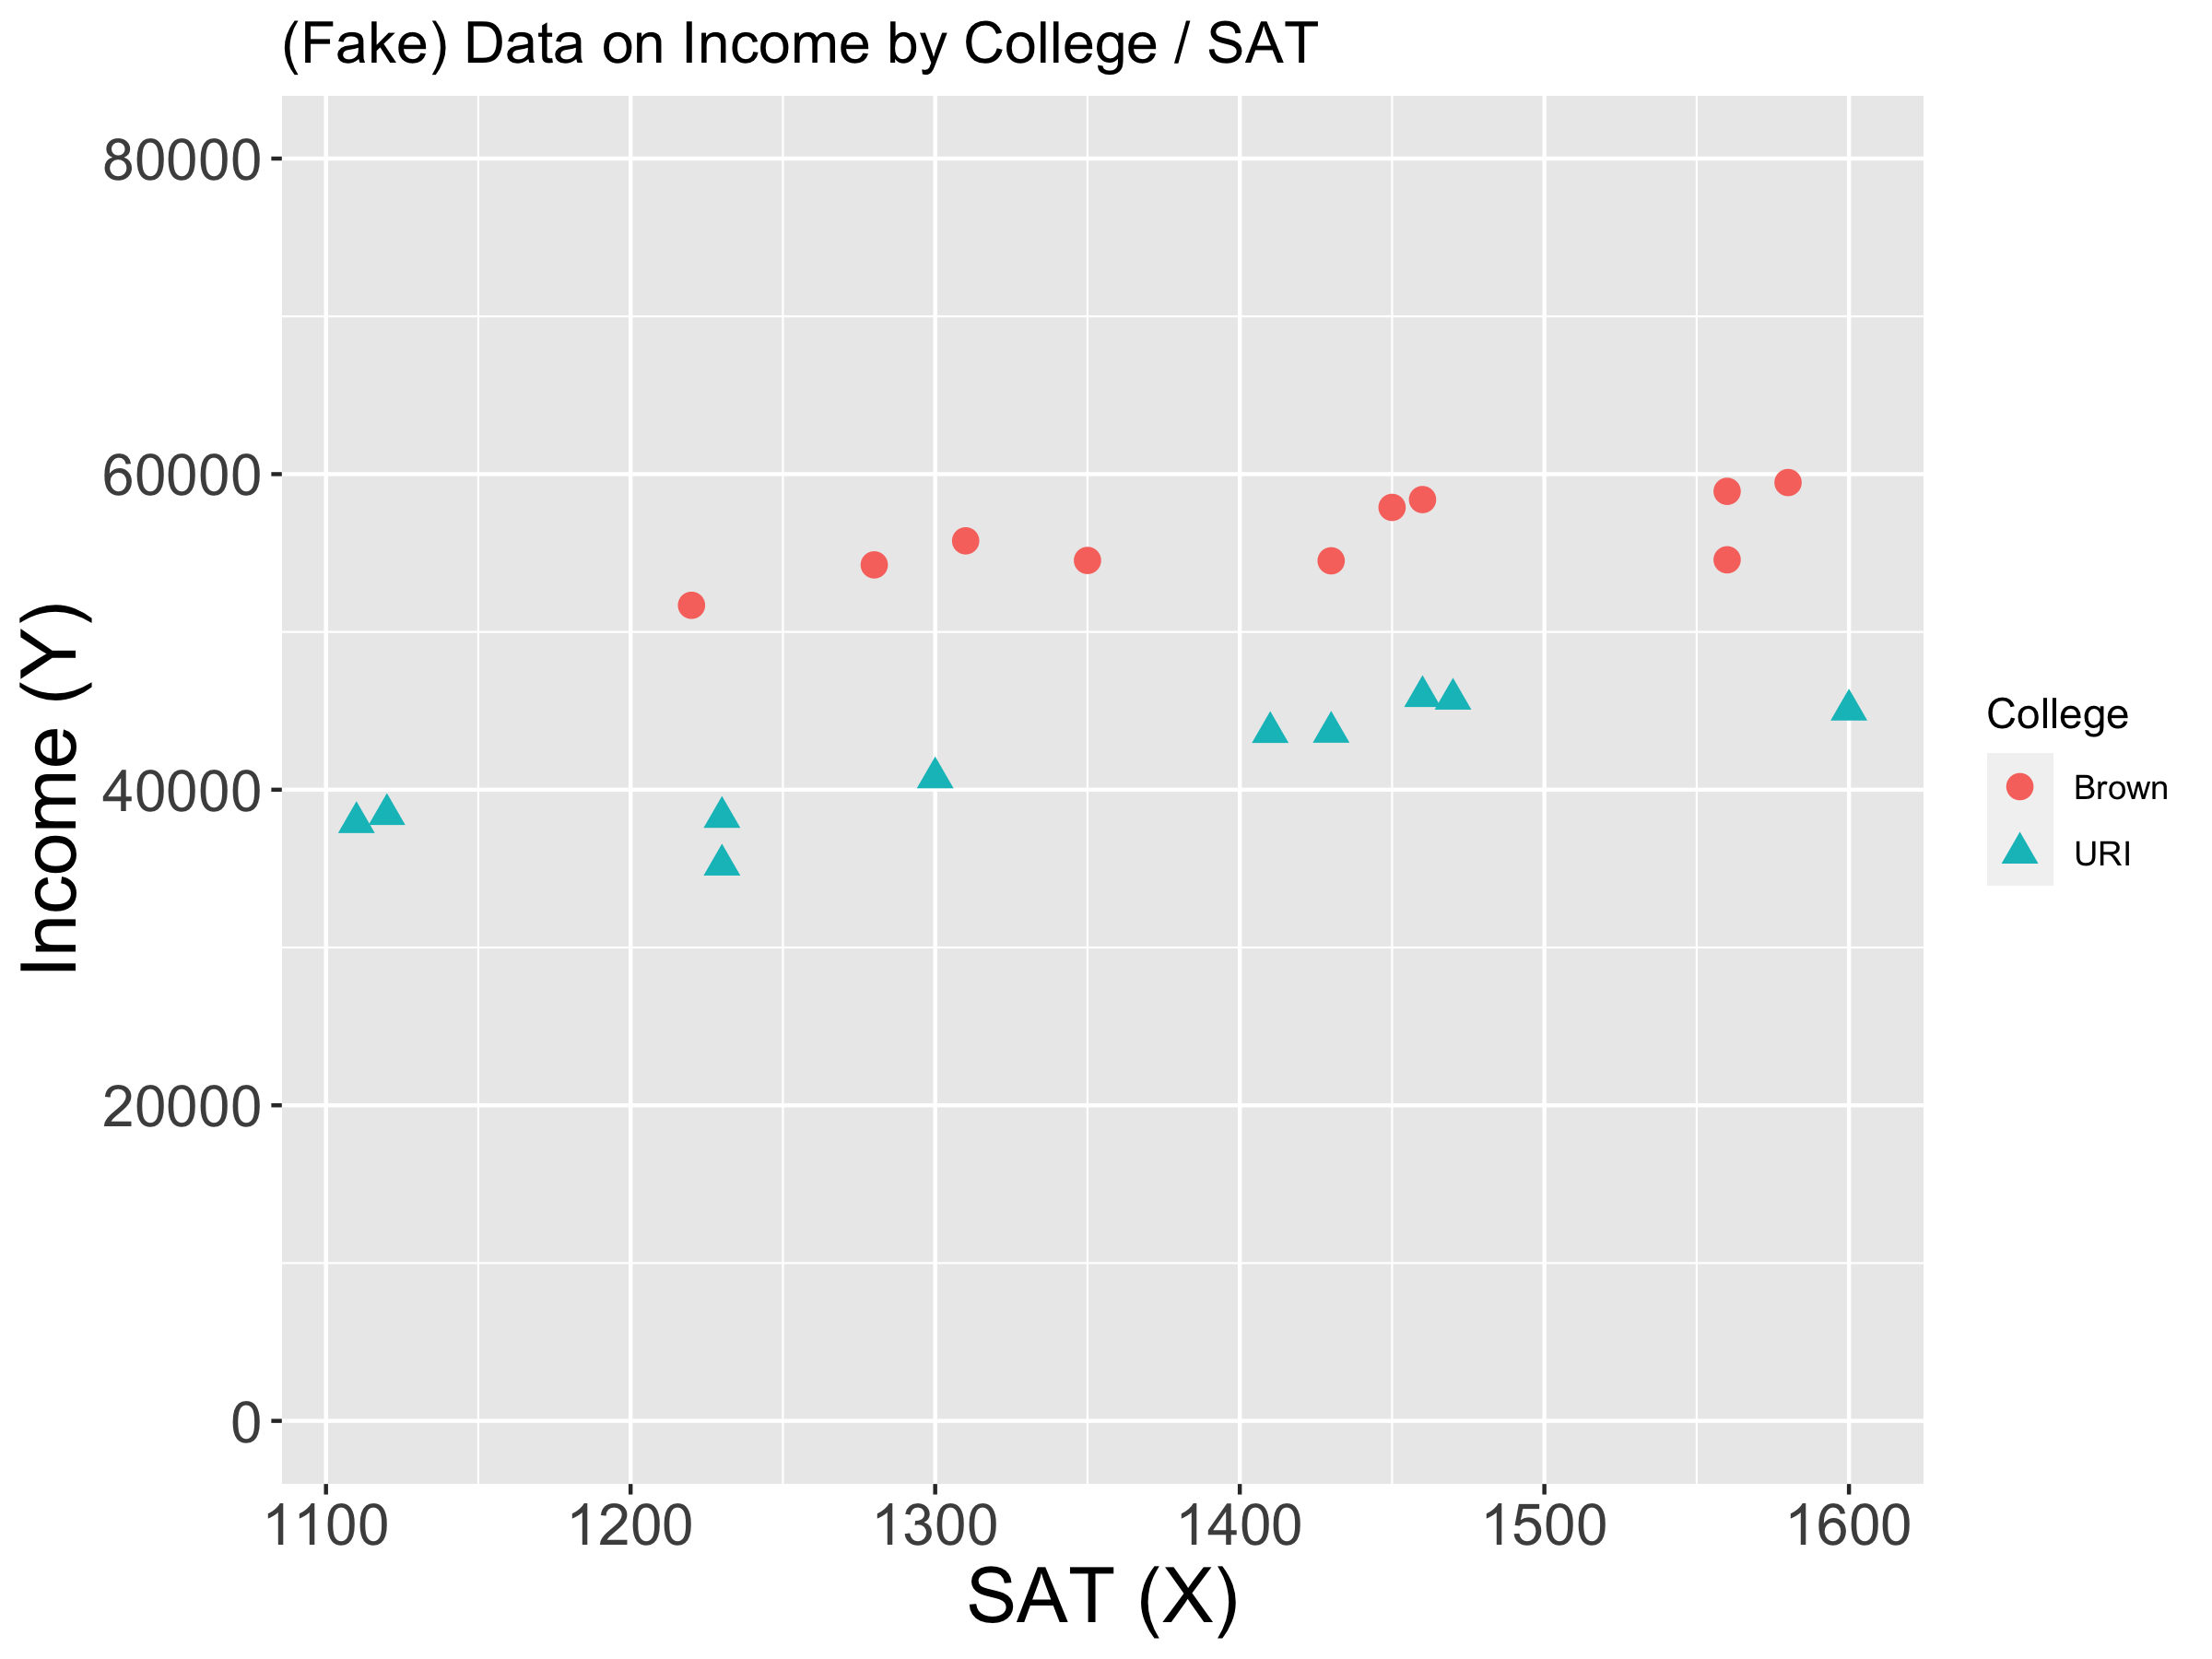
\includegraphics[scale=0.1]{fake-sat.png}}
\only<8>{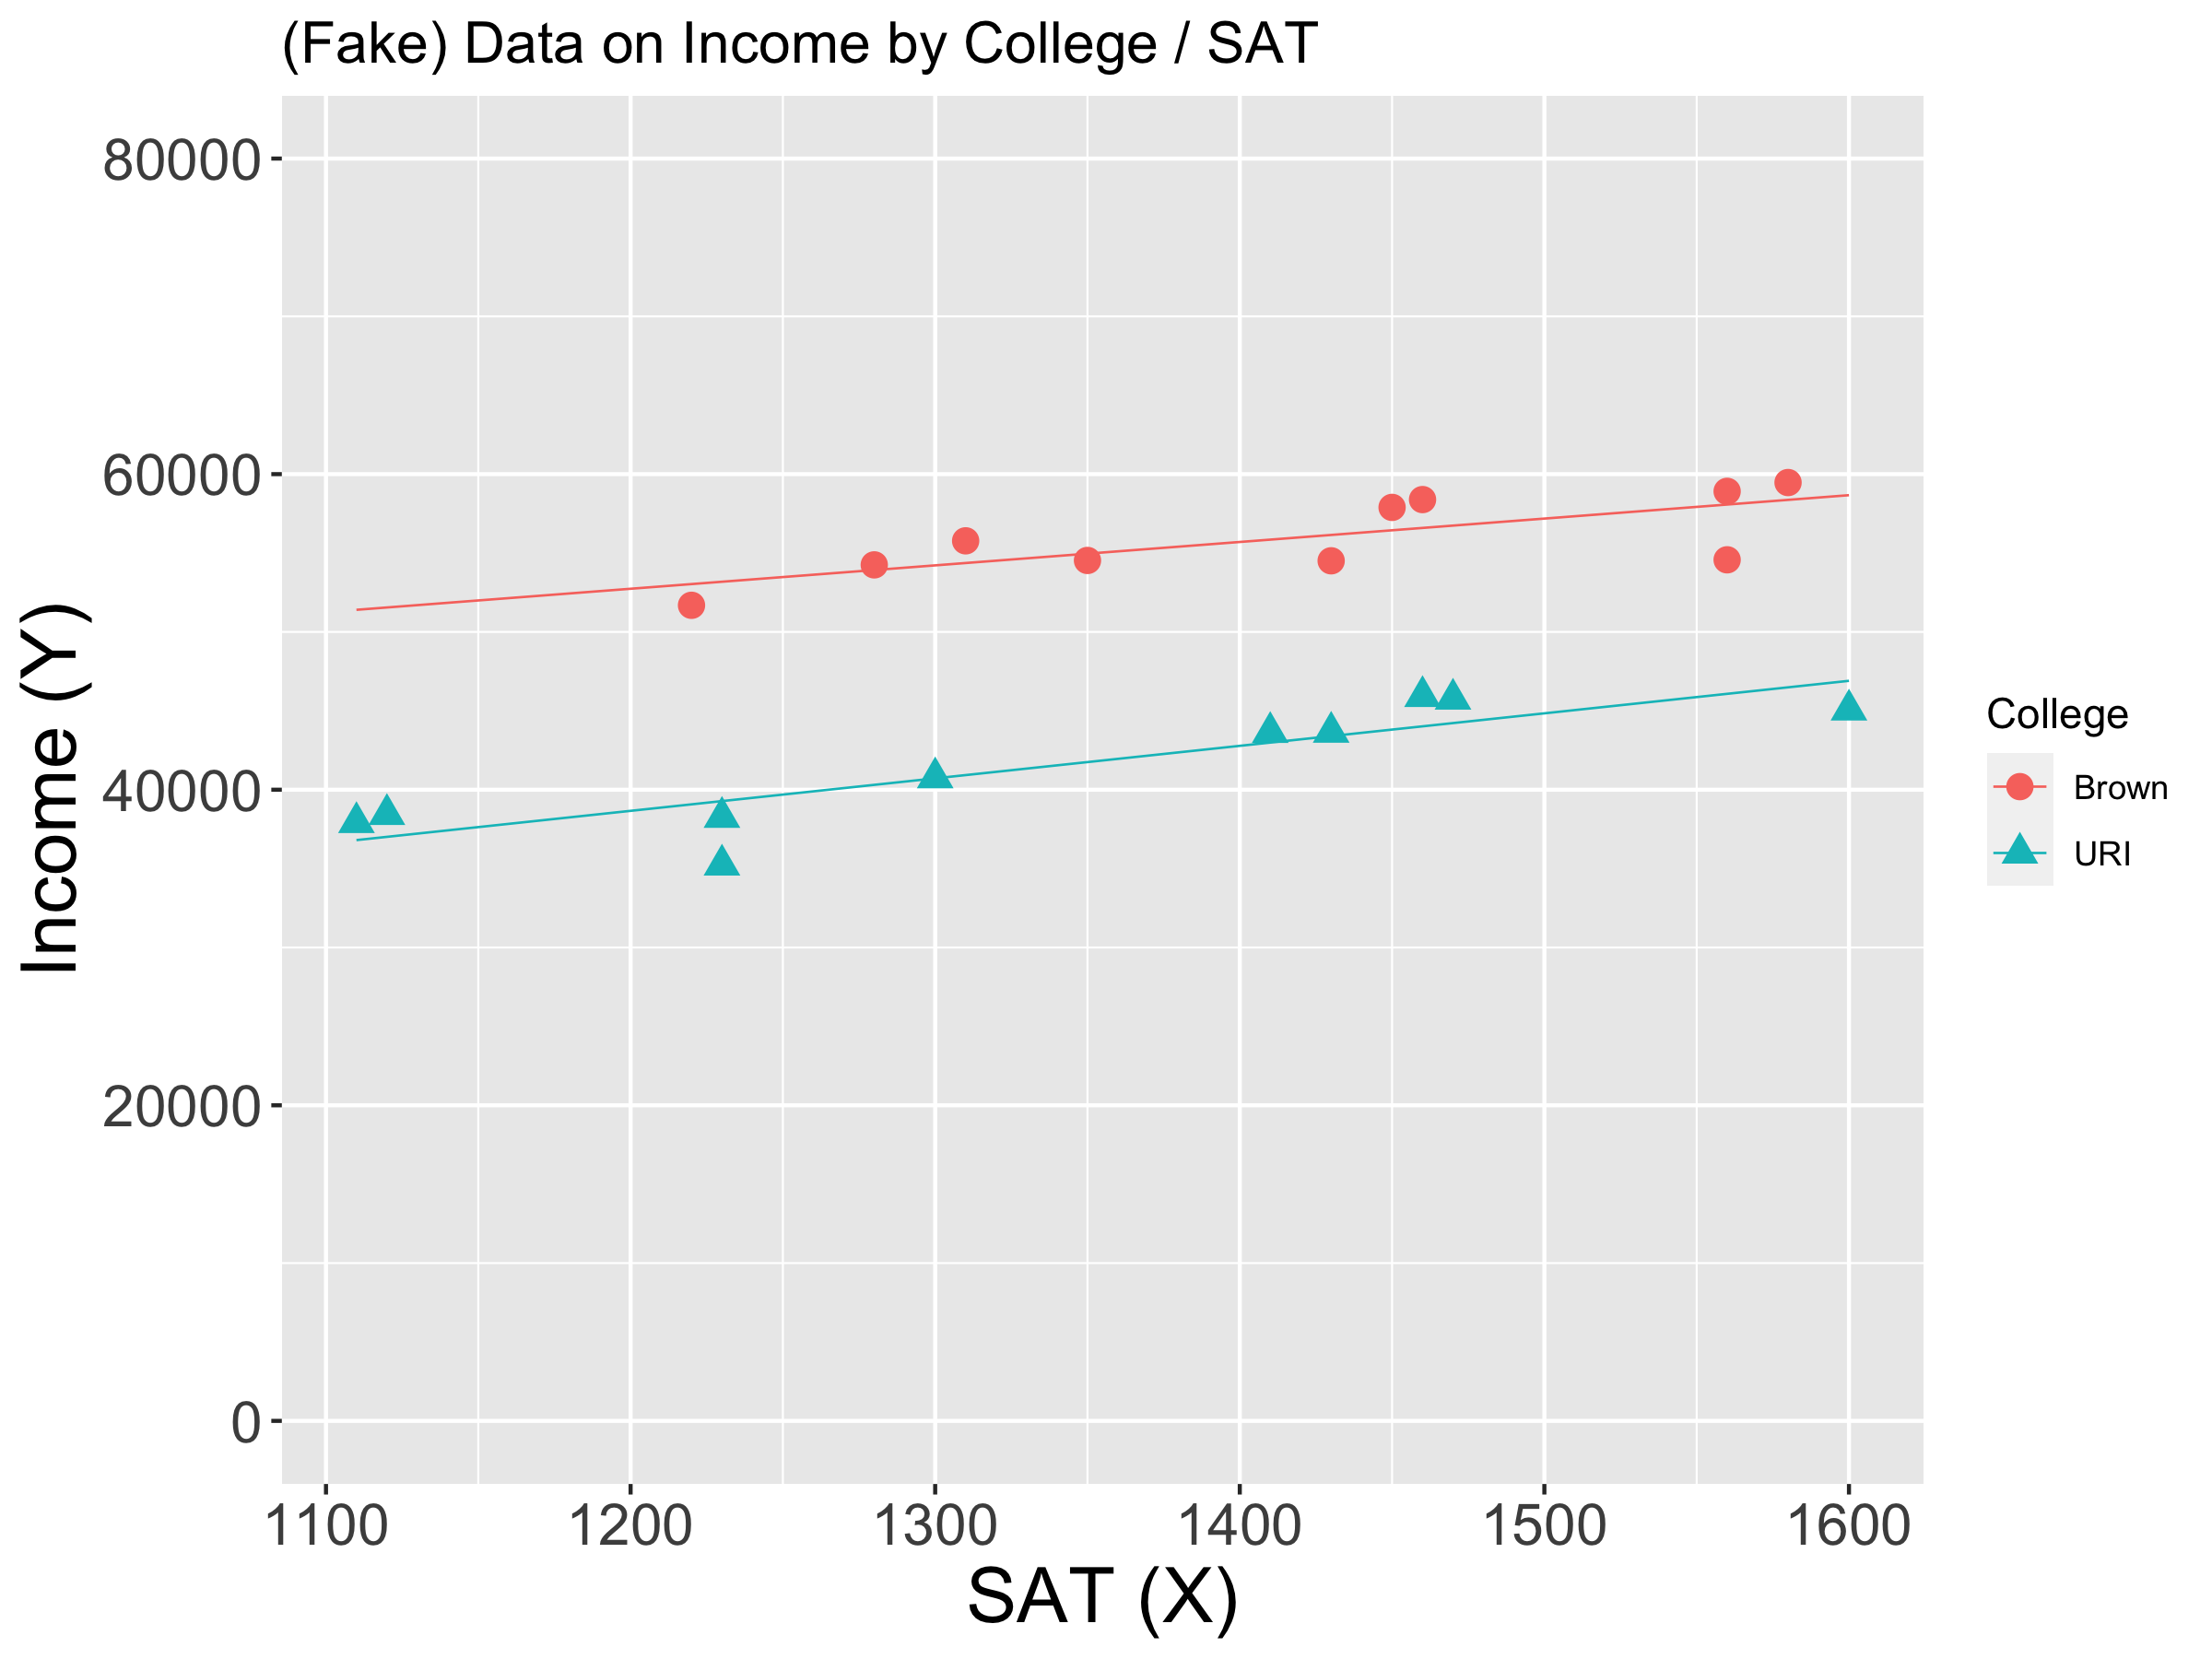
\includegraphics[scale=0.1]{fake-sat-with-trend.png}}
\only<9>{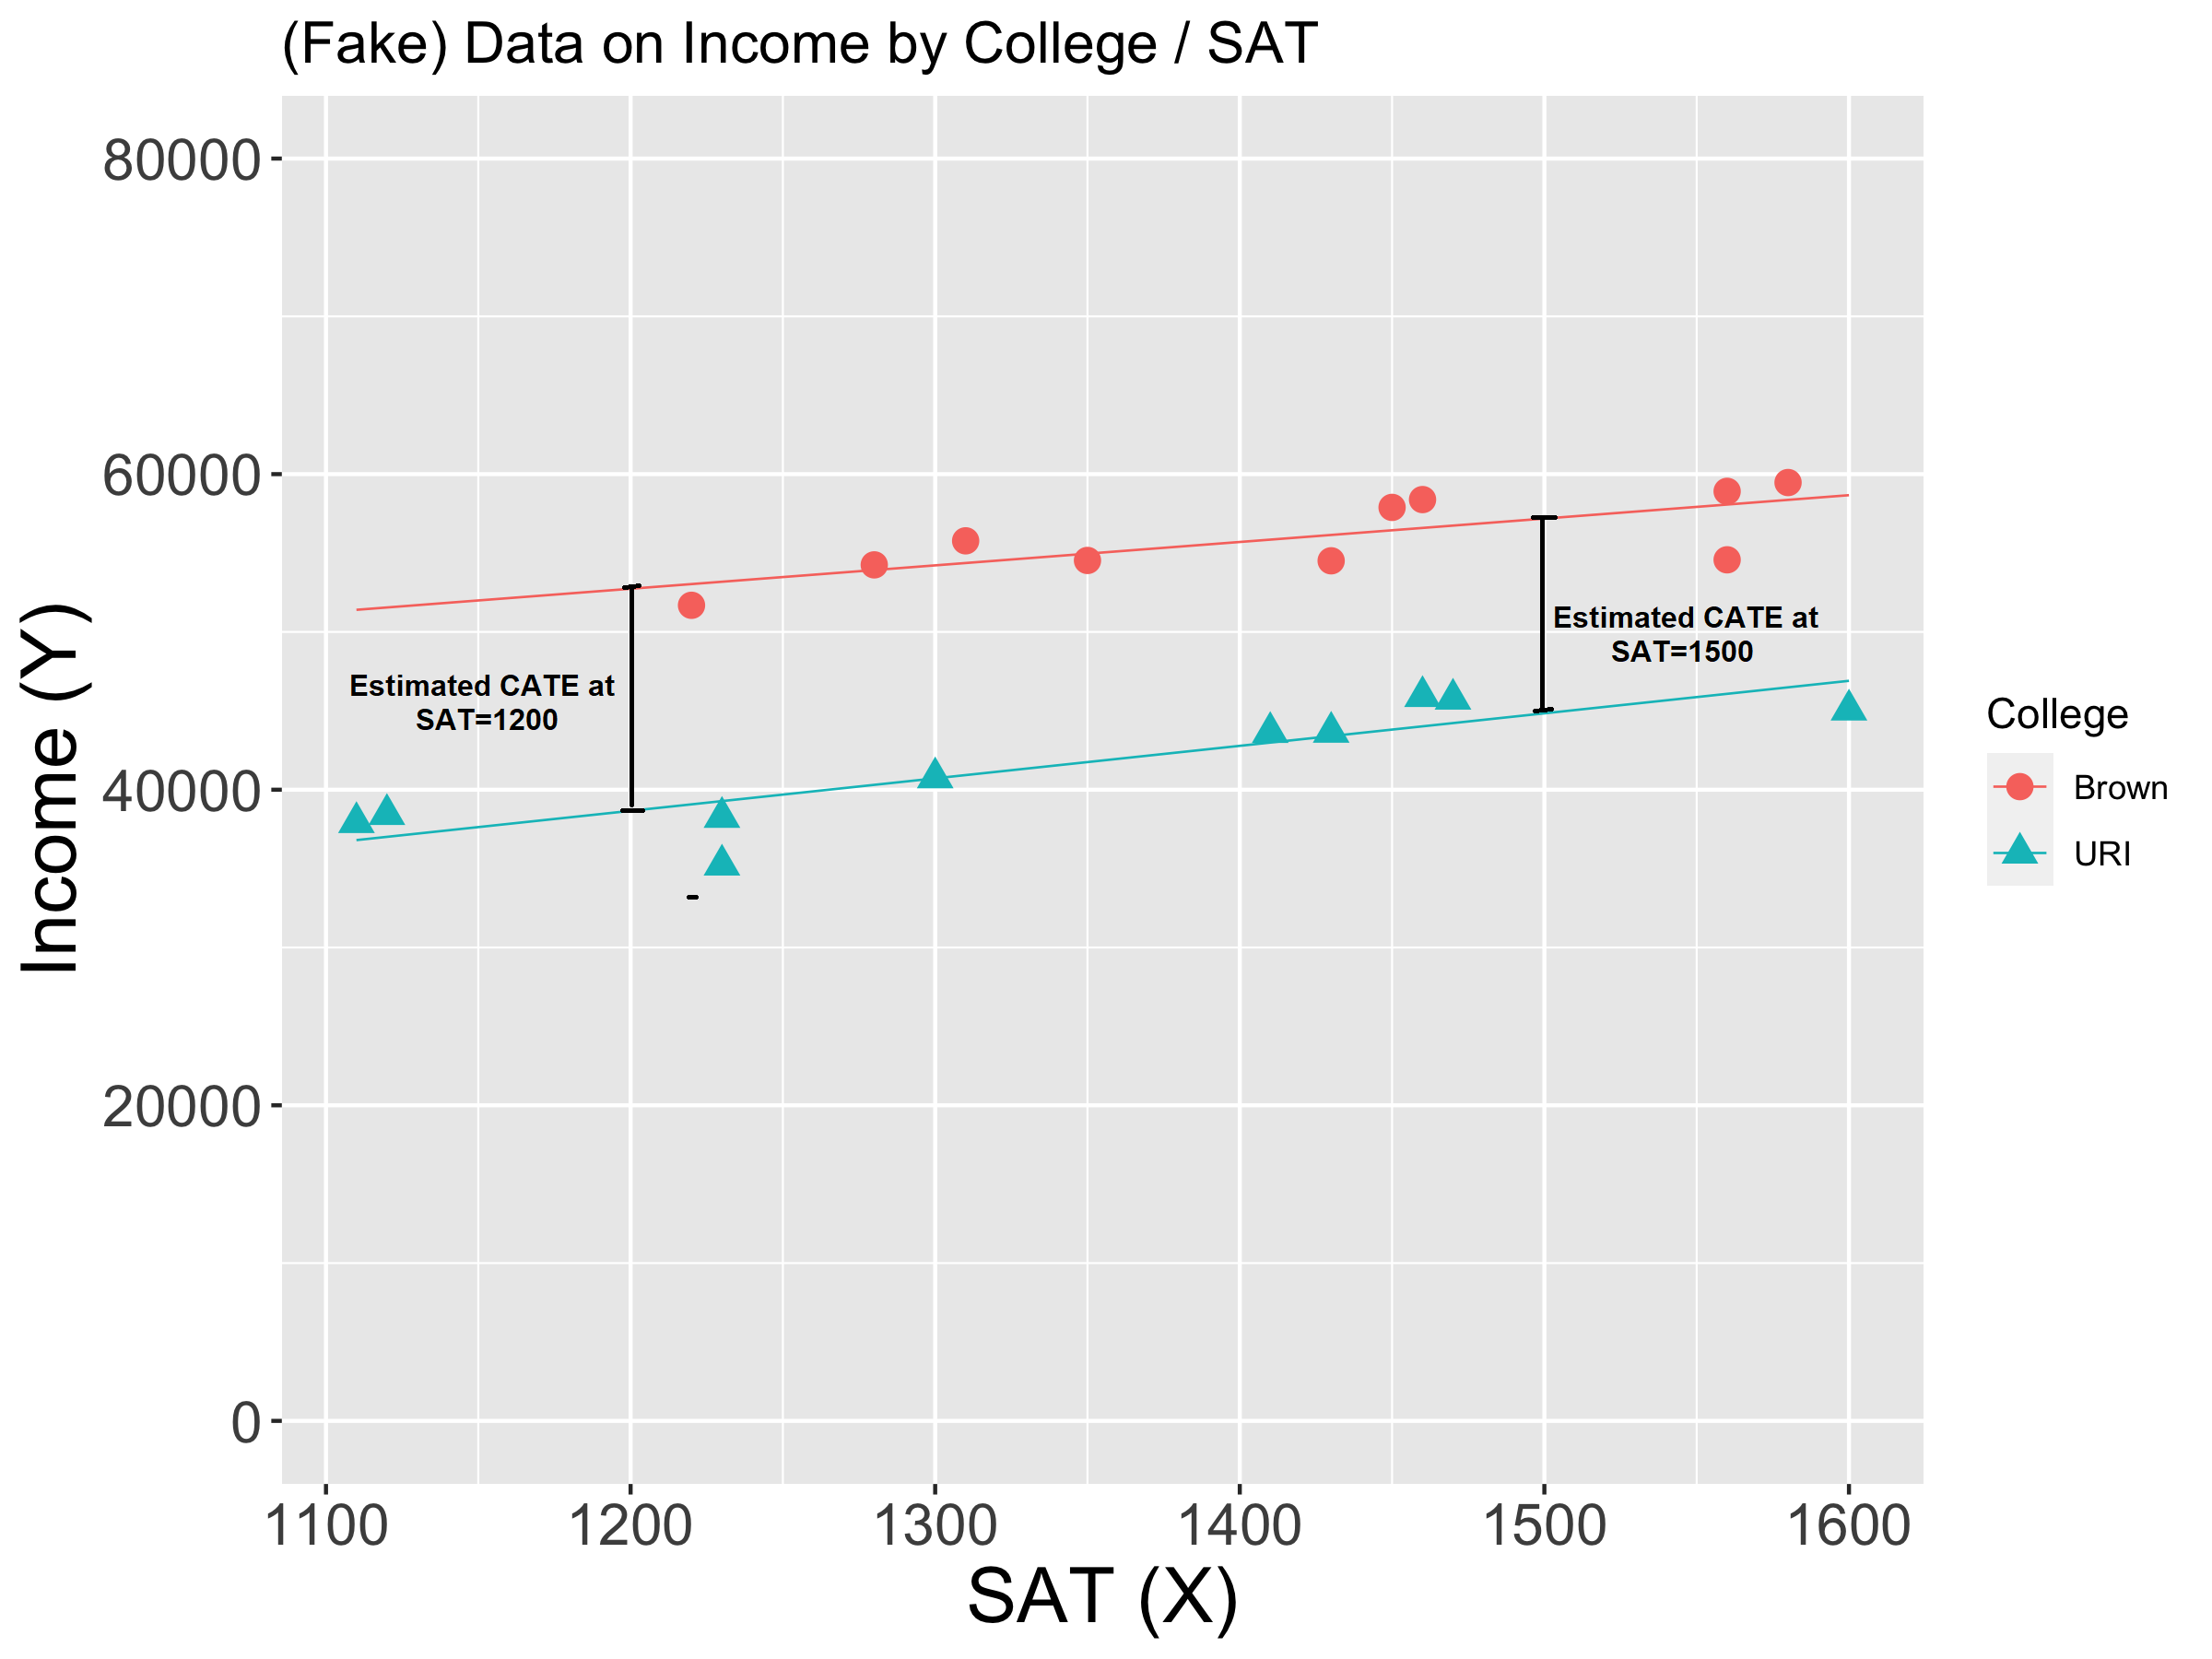
\includegraphics[scale=0.1]{fake-sat-with-trend-annotated2.png}}

\begin{wideitemizeshort}
\only<1> {\item
Imagina que es nuestra data }

\only<2>{
	\item
	Estamos dispuestos a asumir que el puntaje del examen SAT es casi tan bueno como aleatorio
}

\only<3>{
\item	
Imagina que estamos interesados en el efecto (condicional) en $X=1350$. La teoría nos diría que comparemos colegios con puntaje $X=1350$. 
}

\only<4-5>{
\item
Podemos estimar el efecto promedio usando la única observación que tenemos para Brown en $X=1350$. Este estimado es muy ruidoso, \& no podemos usar CLT
}
\smallskip

\only<5>{
\item
Peor aún, no tenemos alumnos de URI con $X=1350$!
}

\only<6-8>{
\item
¡¡Necesitamos extrapolar!!

\pause\smallskip
\item<7-8>
¿Qué haríamos más o menos al ojo? 
\item<8>\smallskip
Dibujar quizás una linea que represente bien en promedio
}

\item<9>
Con esto podemos estimar el efecto promedio $CATE(x)$ en cualquier $x$
\end{wideitemizeshort}
\end{frame}


\begin{frame}{Introducción a la Regresión}
\begin{wideitemize}

\item
La idea de \textbf{regresión} es formalizar el proceso de estimar la función de esperanza condicional (CEF) al extrapolar a través de unidades usando una forma de función específica  (por ej. linear, quadratic, etc.)

\pause
\item
Falta responder:

\pause
\item
¿Cómo aproximar el CEF en la muestra que tenemos? (I.e. como hiciste ese dibujito!)

\pause
\item
¿Cómo construir intervalos de confianza/hipótesis test para estimados del CEF? 

\pause
\item
¿Qué pasa si el CEF no es lineal?

\pause
\item
Ok, tratemos de contestar estas cosas

\end{wideitemize}	
\end{frame}	


\begin{frame}{Camino}
\vspace{0.2cm}
\begin{wideitemize}
\item \textbf{Lo que sabemos hacer:} Estimar y hacer test de hipótesis de medias poblacionales usando promedios muestrales
\item \textbf{Queremos hacer:} Estimar aproximación de CEF y hacer test de hipótesis
\end{wideitemize}
\pause
\bigskip
¿Cómo empezar? 
\pause
\begin{wideitemize}
	\item 1) Asumir CEF toma cierta forma, por ej. lineal:
	$$E[Y_i | X_i = x] = \alpha + x \beta$$
	
	\pause
	\item 2) Mostrar que, $\alpha$ and $\beta$ can  se pueden representar como medias poblacionales
	
	\pause
	\item
	3) Estimar eso con promedio muestral $\alpha,\beta$ y hacer test de hipótesis
	
	\pause
	\item
	4) Argumentar que incluso si CEF no es lineal, $\alpha$ y $\beta$ proveen una buena aproximación
\end{wideitemize}

\end{frame}


\begin{frame}{El ``Least Squares'' Problem}

\begin{wideitemize}

\item
Suponer que $X_i$ es escalar y CEF lineal (se puede relajar luego):
$$E[Y_i | X_i = x] = \alpha + x \beta$$

\pause
\item
Algo útil que se puede explotar es que si la ecuación de arriba es cierta, entonces $(\alpha,\beta)$ solve the ``least squares'' problem:

$$(\alpha,\beta)=\arg\min_{a,b} E[ (Y_i - (a + b X_i))^2  ] $$


\pause
\item
¿De dónde viene esto?

\end{wideitemize}
	
\end{frame}

\begin{frame}{Un problema más simple}
\begin{wideitemize}
	\item
	Antes de mostrar que $(\alpha,\beta)$ resuelve el ``least-squares'' problem, consideremos un problema más sencillo:
	
	\pause
	\item
	Imaginen que queremos encontrar una constante $u$ para minimizar
	$$\min_u E[ (Y_i - u)^2 ]$$
	
	\pause
	\item
	¿Qué constante $u$ deberiamos elegir? \pause La media poblacional $\mu=E[Y_i]$!
	
	\pause
	\item
	Prueba: \\
	
	La derivada de $E[ (Y_i - u)^2 ]$ con respecto a $u$ es $E[ 2(Y_i - u) ]$.  \\ \pause
	
	
Igualando la derivada a cero nos da
	$$E[ 2(Y_i - \mu) ] = 0 \Rightarrow 2 E[Y_i] = 2 u \Rightarrow u = E[Y_i].$$
	
\end{wideitemize}	
\end{frame}

\begin{frame}{Un problema ligeramente más difícil}
\vspace{0.2cm}
\begin{wideitemize}

	\item
	Ahora queremos una función de predicción que dependa de x, $u(x)$, que minimice
	$$\min_{u(\cdot)} E[ (Y_i - u(X_i))^2  ]$$
	
	\pause
	\item
	¿Qué función $u(x)$ usar? \pause La esperanza condicional $u(x) = E[Y|X= x]$. 
	
	\pause
	\item
	Prueba: \\
	Por LIE,
	$$E[ (Y_i - u(X_i))^2  ] = E[  E[  (Y_i - u(X_i)) ^2| X_i  ]   ] .$$
	
	\pause
	Entonces, para cada valor  $x$, queremos elegir $u(x)$ tal que minimice
	$$E[ (Y_i - u(x))^2 | X_i = x ].$$ 
	
	\pause Sin embargo, nuestro argumento en la slide anterior implica que la solución es dada por $u(x) = E[Y_i | X_i = x]$. 
\end{wideitemize}
\end{frame}

\begin{frame}{Regresando\dots}
	
\begin{wideitemize}

\item
Hemos mostrado que $u(x) = E[Y_i | X_i = x]$ resuelve
$$\min_{u(\cdot)} E[ (Y_i - u(X_i))^2  ]$$

\pause
\item
Entonces, si $E[Y_i | X_i = x] = \alpha + \beta x$, entonces $u(x) = \alpha + \beta x$ minimiza  
$$\min_{u(\cdot)} E[ (Y_i - u(X_i))^2  ]$$

\pause
\item
La minimización de arriba es sobre \textit{todas} las funciones $u(\cdot)$, incluyendo las lineales $a + b x$. Por tanto, 

$$ E[ (Y_i -  (\alpha + \beta X_i)  )^2  ] \leq  E[ (Y_i -  (a + b X_i)  )^2  ]  \text{ para todo } a ,b. $$

\pause
\item
Esto implica que $(\alpha,\beta)$ resuelve

$$\min_{a,b}E[ (Y_i -  (a+ b X_i)  )^2  ] ,$$

\noindent tal como queriamos mostrar
\end{wideitemize}	
\end{frame}


\begin{frame}{¿Por qué es útil esto?}
\begin{wideitemize}

\item
Hemos mostrado que $\alpha,\beta$ solucionan 

$$\min_{a,b}E[ (Y_i -  (a+ b X_i)  )^2  ] .$$

\item 
¿En qué ayuda esto? \pause Resolviendo esto podemos expresar $\alpha,\beta$ como funciones de la población 

\pause
\item
Derivemos con respecto  $a$ y $b$ e igualamos a cero en ambos $(\alpha,\beta)$: \pause
\begin{align*}
& E[-2  (Y_i - (\alpha + \beta X_i )) ] = 0 \\ \pause
& E[-2  X_i (Y_i -(\alpha + \beta X_i)) ] = 0
\end{align*}

\pause
\item
Tenemos 2 ecuaciones, 2 incógnitas, podemos resolver para $(\alpha,\beta)$

\end{wideitemize}
\end{frame}

\begin{frame}{La solución Least Squares}
\begin{wideitemize}
\item
La solución al sistema es 
\begin{align*}
& \beta = \frac{E[ (X_i -E[X_i]) (Y_i - E[Y_i])  ]}{E[ (X_i - E[X_i])^2 ]} = \frac{Cov(X_i, Y_i)}{Var(X_i)} \\ 
& \alpha = E[Y_i] - E[X_i] \beta
\end{align*}

\pause
\item
Son funciones continuas de medias poblacionales!

\pause
\item
Podemos usar las técnicas anteriores para estimar y hacer test de hipótesis sobre el CEF!
\end{wideitemize}	
\end{frame}



\begin{frame}{Estimando Coeficientes de Regresión}
	\begin{wideitemize}
	\item
	Mostramos que $E[Y_i\mid X_i=x]=\alpha+\beta x$
\begin{align*}
& \beta = \frac{E[ (X_i -E[X_i]) (Y_i - E[Y_i])  ]}{E[ (X_i - E[X_i])^2 ]} = \frac{Cov(X_i, Y_i)}{Var(X_i)} \\ 
& \alpha = E[Y_i] - E[X_i] \beta
\end{align*}
	
	\item
	¿Cómo estimar $\alpha,\beta$? \pause \\ Medias poblacionales por promedios muestrales
	\pause
	\begin{align*}
		& \hat\beta = \dfrac{ \frac{1}{N} \sum_{i=1}^{N} (X_i - \bar{X})(Y_i - \bar{Y})  }{ \frac{1}{N} \sum_{i=1}^N (X_i - \bar{X})^2 } =\frac{\widehat{Cov}(X_i,Y_i)}{\widehat{Var}(X_i)}\pause{} \\
		& \hat\alpha = \bar{Y} - \bar{X} \hat{\beta}
	\end{align*}

	
	\pause
	\item
	Estos $\hat\alpha,\hat\beta$ se llaman  coeficientes de \textit{ordinary least squares} (OLS) \smallskip
\begin{itemize}
\item Resuelven el problema análogo en la muestra, $\min_{a,b}\frac{1}{N}\sum_i (Y_i -  (a+ b X_i)  )^2   $
\end{itemize}
	\end{wideitemize}	
\end{frame}


\begin{frame}
	\centering
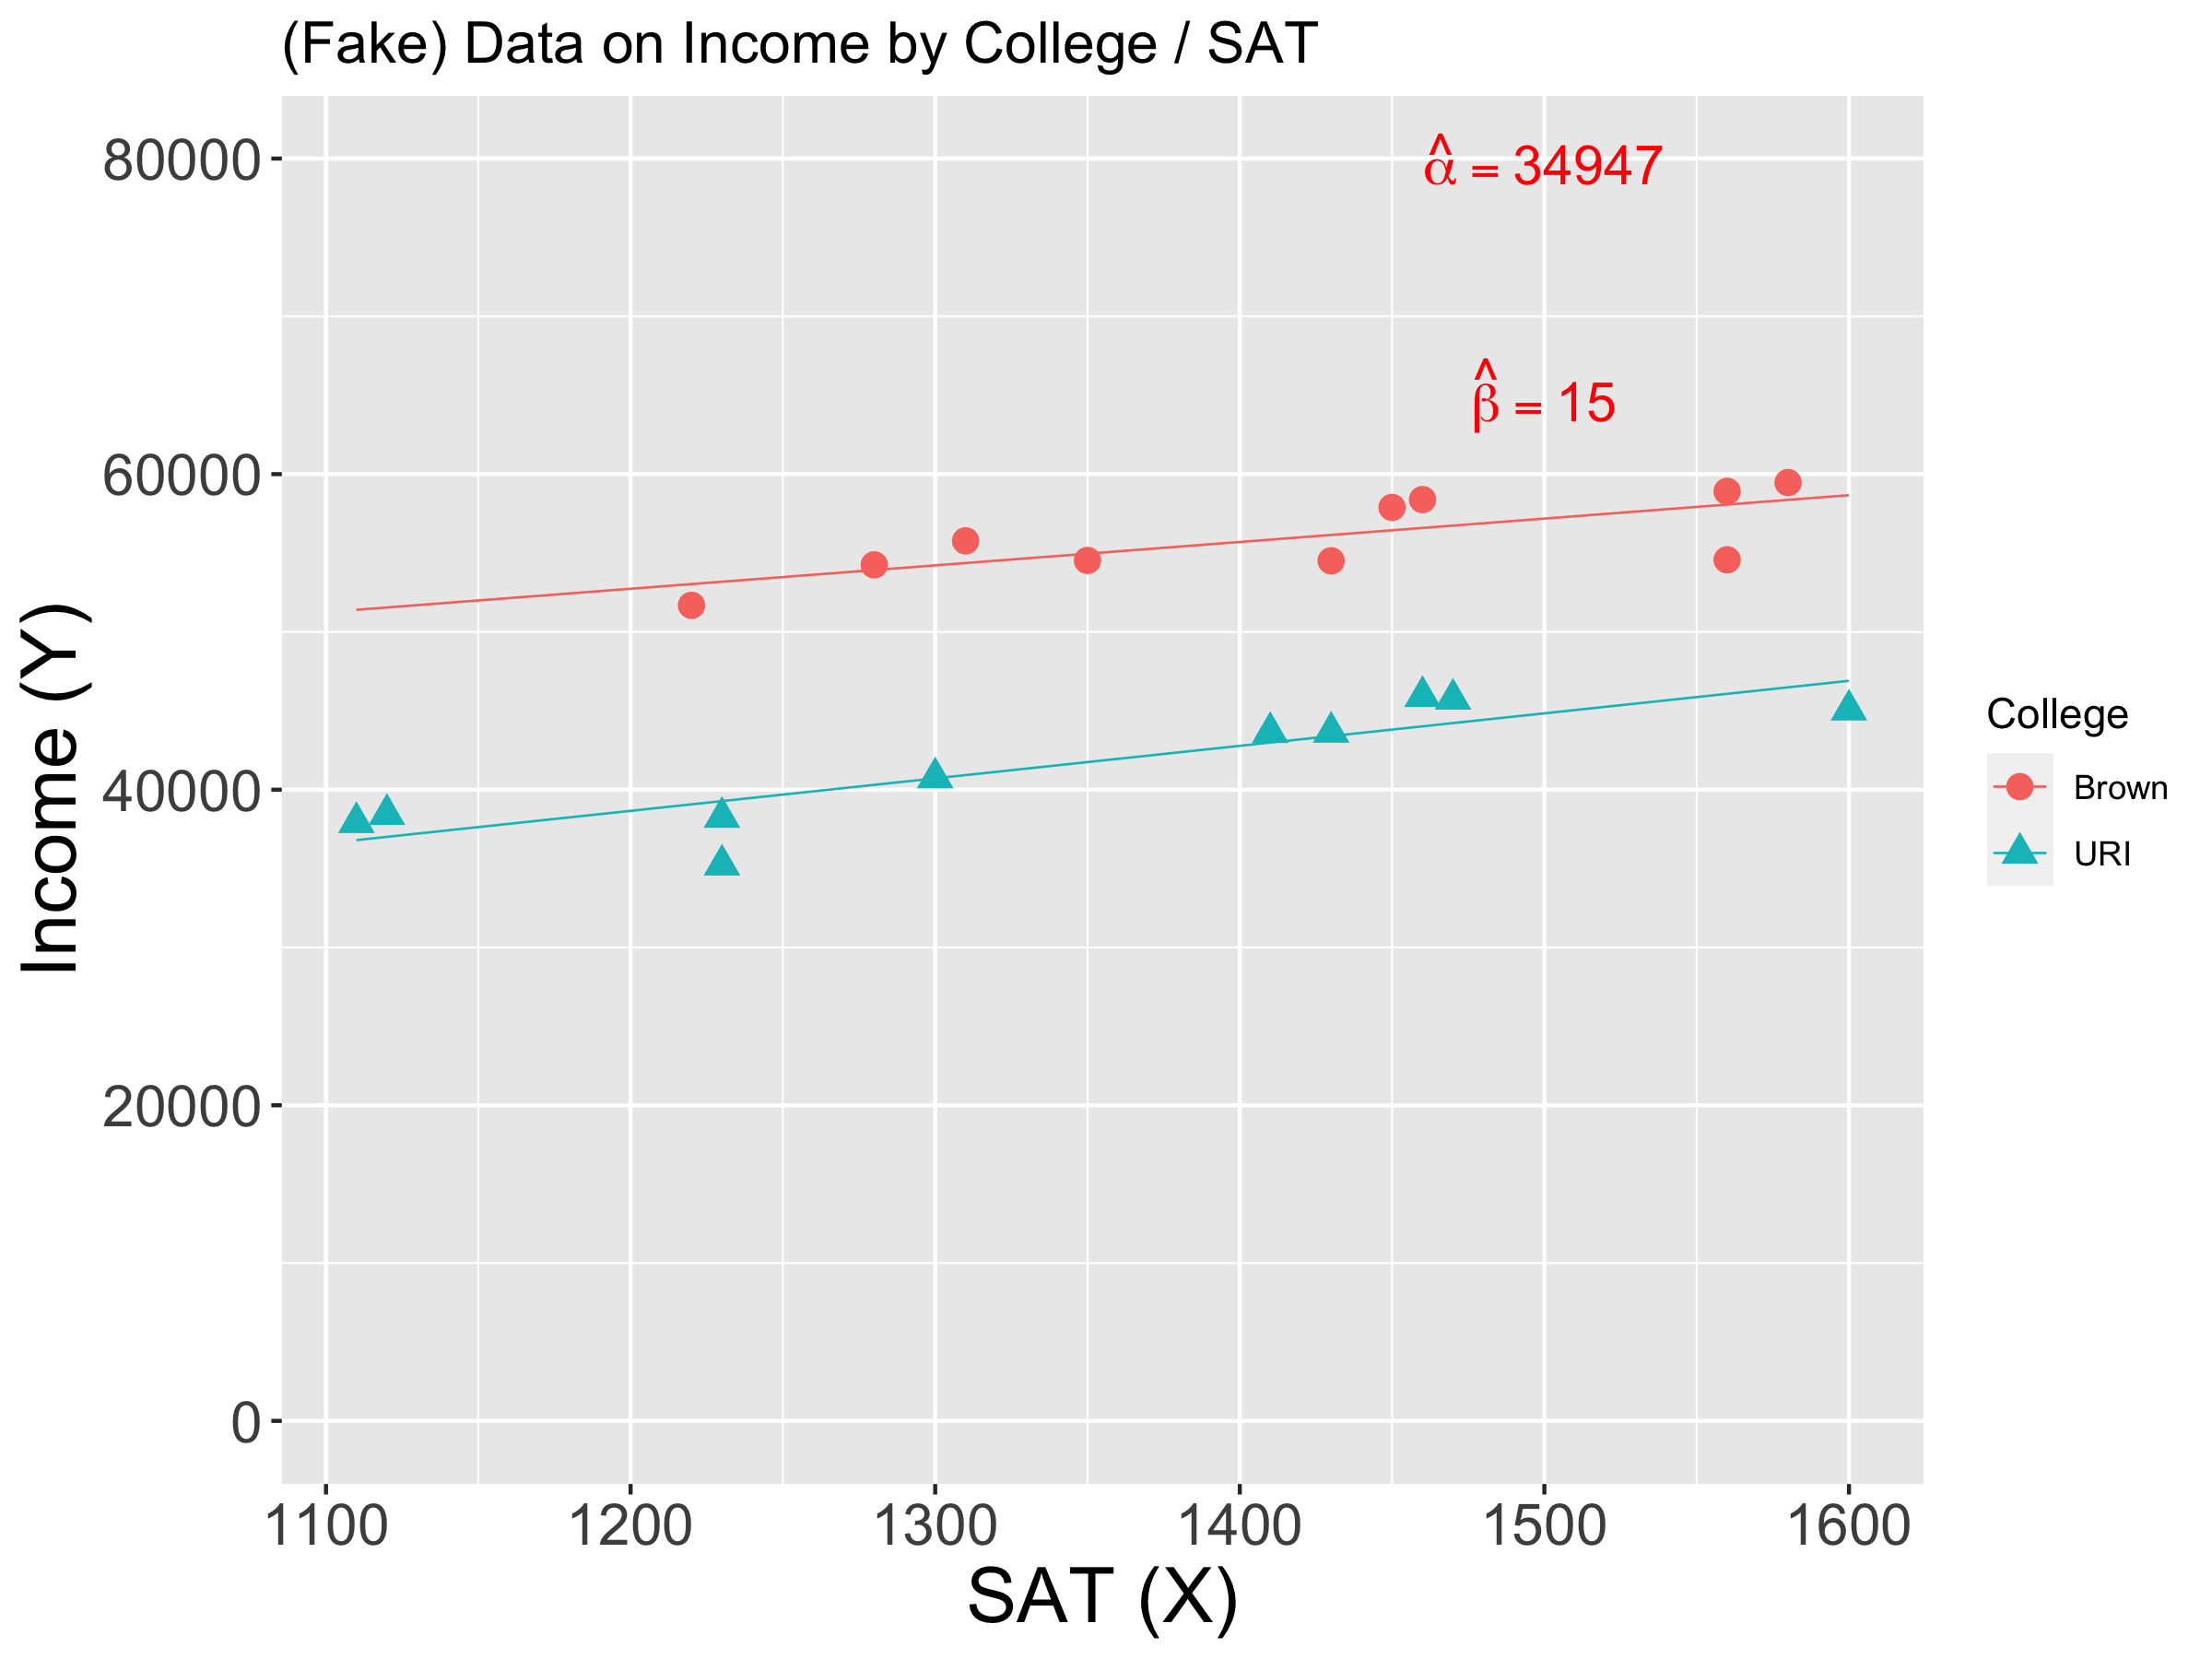
\includegraphics[scale=0.1]{fake-sat-with-trend-brown-betas.png}
\end{frame}

\begin{frame}
	\centering
	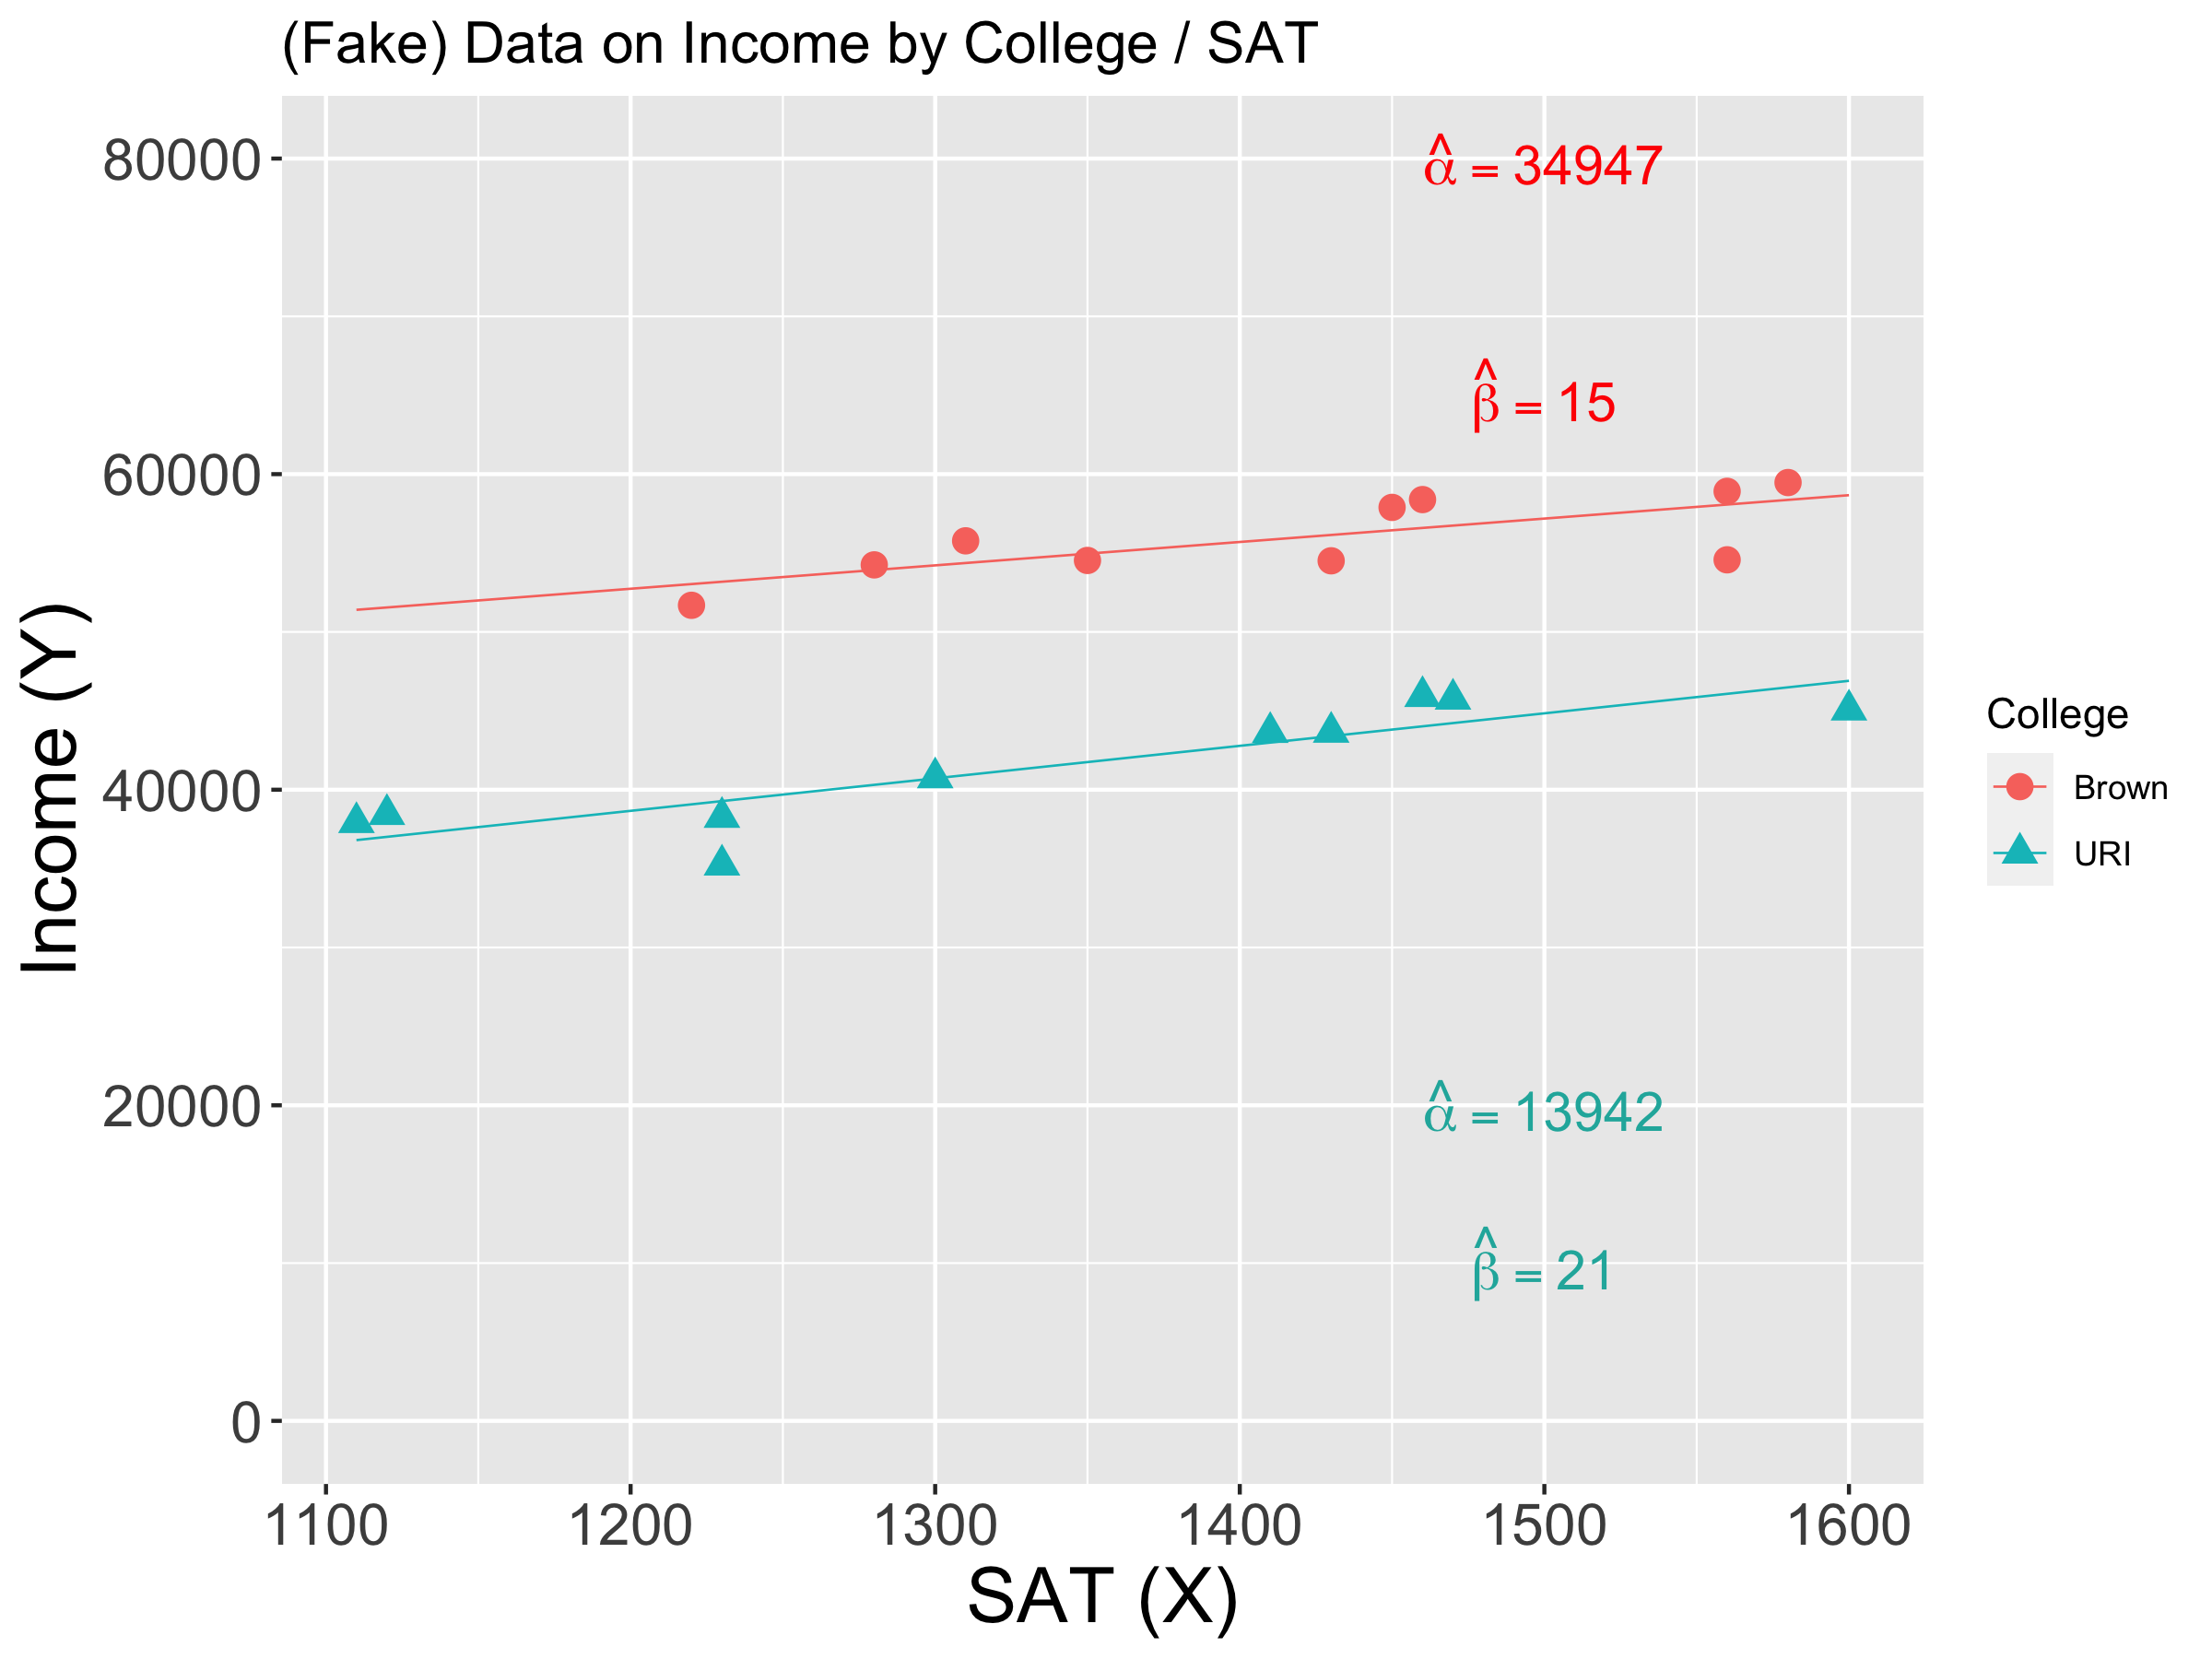
\includegraphics[scale=0.1]{fake-sat-with-trend-both-betas.png}
	
	\pause
	\begin{wideitemize}
		\item
		¿Cuál es el valor estimado de $E[Y_i | D_i = 1, X_i = 1350]$? \pause $\hat\alpha + \hat\beta \cdot 1350 = 34947 + 15 \cdot 1350 = 55197$. 
	\end{wideitemize}
\end{frame}


%\begin{frame}{Estimating $CATE(x)$}
%\begin{wideitemize}
%\item
%Remember that under conditional unconfoundedness: 
%$$CATE(x) = E[ Y_i |D_i = 1, X_i =x ] - E[Y_i |D_i =0, X_i  = x]$$
%
%\item
%Under our assumption that 
%\end{wideitemize}	
%\end{frame}

\begin{frame}{Consistencia de OLS}
\begin{wideitemize}
\item
Podemos usar los resultados que sabemos anteriormente para mostrar que $\hat\beta$ es consistente para $\beta$, i.e. $\hat\beta \rightarrow_p \beta$.

\pause
\item
Tenemos que
\begin{align*}
 \hat\beta &=\left( \frac{1}{N} \sum_{i=1}^N (X_i - \bar{X})^2 \right)^{-1}   \frac{1}{N} \sum_{i=1}^{N} (X_i - \bar{X})(Y_i - \bar{Y}) \pause{}  \\
 &= \left( \frac{1}{N} \sum_{i=1}^N X_i^2 - \bar{X}^2 \right)^{-1}   \left( \frac{1}{N} \sum_{i=1}^{N} X_i Y_i - \bar{X} \bar{Y} \right) \pause{} \\
 & \rightarrow_p \left( E[X_i^2] - E[X_i]^2 \right)^{-1}   \left( E[X_i Y_i] - E[X_i] E[Y_i] \right) \pause{} \\
 &= Var(X_i)^{-1} Cov(X_i, Y_i) \pause{} = \beta
\end{align*}


\pause
\item
De la misma manera, podemos mostrar que $\hat\alpha \rightarrow_p \alpha$.
\end{wideitemize}		
\end{frame}


\begin{frame}{Distribución Asintótica de OLS}
	\begin{wideitemize}
	\item
	Los estimados $\hat\alpha, \hat\beta$ son funciones continuas de medias muestrales
	
	\pause
	\item
	Podemos usar el CLT y CMT para mostrar que están asintóticamente normalmente distribuidas	
	\pause
	\item
	En particular, podemos mostrar que
	
		$$\sqrt{N}(\hat\beta - \beta) \rightarrow_d N(0, \sigma^2),$$
	
	\noindent donde
	
	$$\sigma^2 = \dfrac{  Var((X_i - E[X_i])\epsilon_i) }{ Var(X_i)^2  }$$ 
	
	
	\pause
	\item
	Esto es útil porque podemos crear CIs para $\beta$ de la forma $\hat\beta 	\pm 1.96 \hat\sigma / \sqrt{N}$, donde $\hat\sigma$ es nuestro valor estimado de $\sigma$. 
	
	\end{wideitemize}	
\end{frame}

\begin{frame}{Derivando Distribución Asintótica de OLS}
\begin{wideitemize}

\item
Define el \textbf{residual} $\epsilon_i = Y_i - (\alpha+X_i \beta)$, implicando
\begin{equation*}
Y_i = \alpha + X_i \beta + \epsilon_i	
\end{equation*}

\pause
\item
Las condiciones de primer orden de $(\alpha,\beta)$ implican que el residual tiene media cero, y es \textbf{ortogonal} to the \textbf{regressor}: $E[\epsilon_i] = E[X_i \epsilon_i] =0$

\pause
\item
Tomando promedios, $\bar{Y} = \alpha + \bar{X} \beta + \bar{\epsilon}$. \pause Entonces $Y_i - \bar{Y} = (X_i - \bar{X})\beta + (\epsilon_i-\bar\epsilon)$

\end{wideitemize}

\end{frame}

\begin{frame}{Derivando Distribución Asintótica de OLS (cont.)}
	\begin{wideitemize}
		
		\item
		Acabamos de derivar que $Y_i - \bar{Y} = (X_i - \bar{X})\beta + (\epsilon_i-\bar\epsilon)$. 
		
		\item
		Entonces,
		\begin{align*}
			\hat\beta &=\left( \frac{1}{N} \sum_{i=1}^N (X_i - \bar{X})^2 \right)^{-1}   \frac{1}{N} \sum_{i=1}^{N} (X_i - \bar{X})(Y_i - \bar{Y})   \\
			&=\pause{} \left( \frac{1}{N} \sum_{i=1}^N (X_i - \bar{X})^2 \right)^{-1}   \frac{1}{N} \sum_{i=1}^{N} (X_i - \bar{X})((X_i - \bar{X})\beta + (\epsilon_i-\bar\epsilon) ) \pause{} \\
			& =\beta + \left( \frac{1}{N} \sum_{i=1}^N (X_i - \bar{X})^2 \right)^{-1}   \frac{1}{N} \sum_{i=1}^{N} (X_i - \bar{X}) (\epsilon_i - \bar\epsilon)
		\end{align*}
\end{wideitemize}	
\end{frame}

\begin{frame}{Derivando Distribución Asintótica de OLS (cont.)}
\begin{wideitemize}
	\item	Por tanto,
	\begin{align*}
		\sqrt{N}(\hat\beta - \beta) &= \left( \frac{1}{N} \sum_{i=1}^N (X_i - \bar{X})^2 \right)^{-1}  \sqrt{N} \frac{1}{N} \sum_{i=1}^N (X_i - \bar{X})(\epsilon_i - \bar{\epsilon}) \pause{} \\
		&= \left( \frac{1}{N} \sum_{i=1}^N (X_i - \bar{X})^2 \right)^{-1} \sqrt{N}\frac{1}{N} \sum_{i=1}^N (X_i - E[X_i])\epsilon_i \\
		&-\left( \frac{1}{N} \sum_{i=1}^N (X_i - \bar{X})^2 \right)^{-1}  \left( \bar{\epsilon} \sqrt{N} (\bar{X} - E[X_i]) \right)
	\end{align*}

	\item
	Por LLN y CMT, $\left( \frac{1}{N} \sum_{i=1}^N (X_i - \bar{X})^2 \right)^{-1} \rightarrow_p Var(X_i)^{-1}$
	
	\pause
	\item
	Por CLT, $\sqrt{N}\frac{1}{N} \sum_{i=1}^N (X_i - E[X_i])\epsilon_i \rightarrow_d \mathrm{N}(0, Var((X_i - E[X_i])\epsilon_i)).$
	
	\pause
	\item
	Por LLN, CLT, y Slutsky,  $\bar{\epsilon} \sqrt{N} (\bar{X} - E[X_i]) \rightarrow_d 0 \times \mathrm{N}(0, Var(X_i))  = 0$
	
\end{wideitemize}

\end{frame}

\begin{frame}{Terminando (!)}
	
	\begin{wideitemize}
	\item
	Poniendo las piezas juntas, tenemos que
	
	$$\sqrt{N}(\hat\beta - \beta) \rightarrow_d N(0, \sigma^2),$$
	
	\noindent donde
	
	$$\sigma^2 = \dfrac{  Var((X_i - E[X_i])\epsilon_i) }{ Var(X_i)^2  }$$ 
	
	\item
	Como antes, podemos estimar la varianza $\sigma^2$ usando promedios muestrales,
	
	$$\hat\sigma^2 = \dfrac{  \frac{1}{N} \sum_i ((X_i - \bar{X})\hat\epsilon_i )^2}{ \left(\frac{1}{N} \sum_i (X_i - \bar{X})^2\right)^2  }, \text{ where } \hat\epsilon_i = Y_i - (\hat\alpha + X_i \hat\beta)$$ 
	
	
	\item
	\pause
	Podemos hacer los mismos pasos para mostrar que $\hat\alpha$ también se distribuye de manera normal asintóticamente. 
\end{wideitemize}	
\end{frame}
		
		
\begin{frame}
	\centering
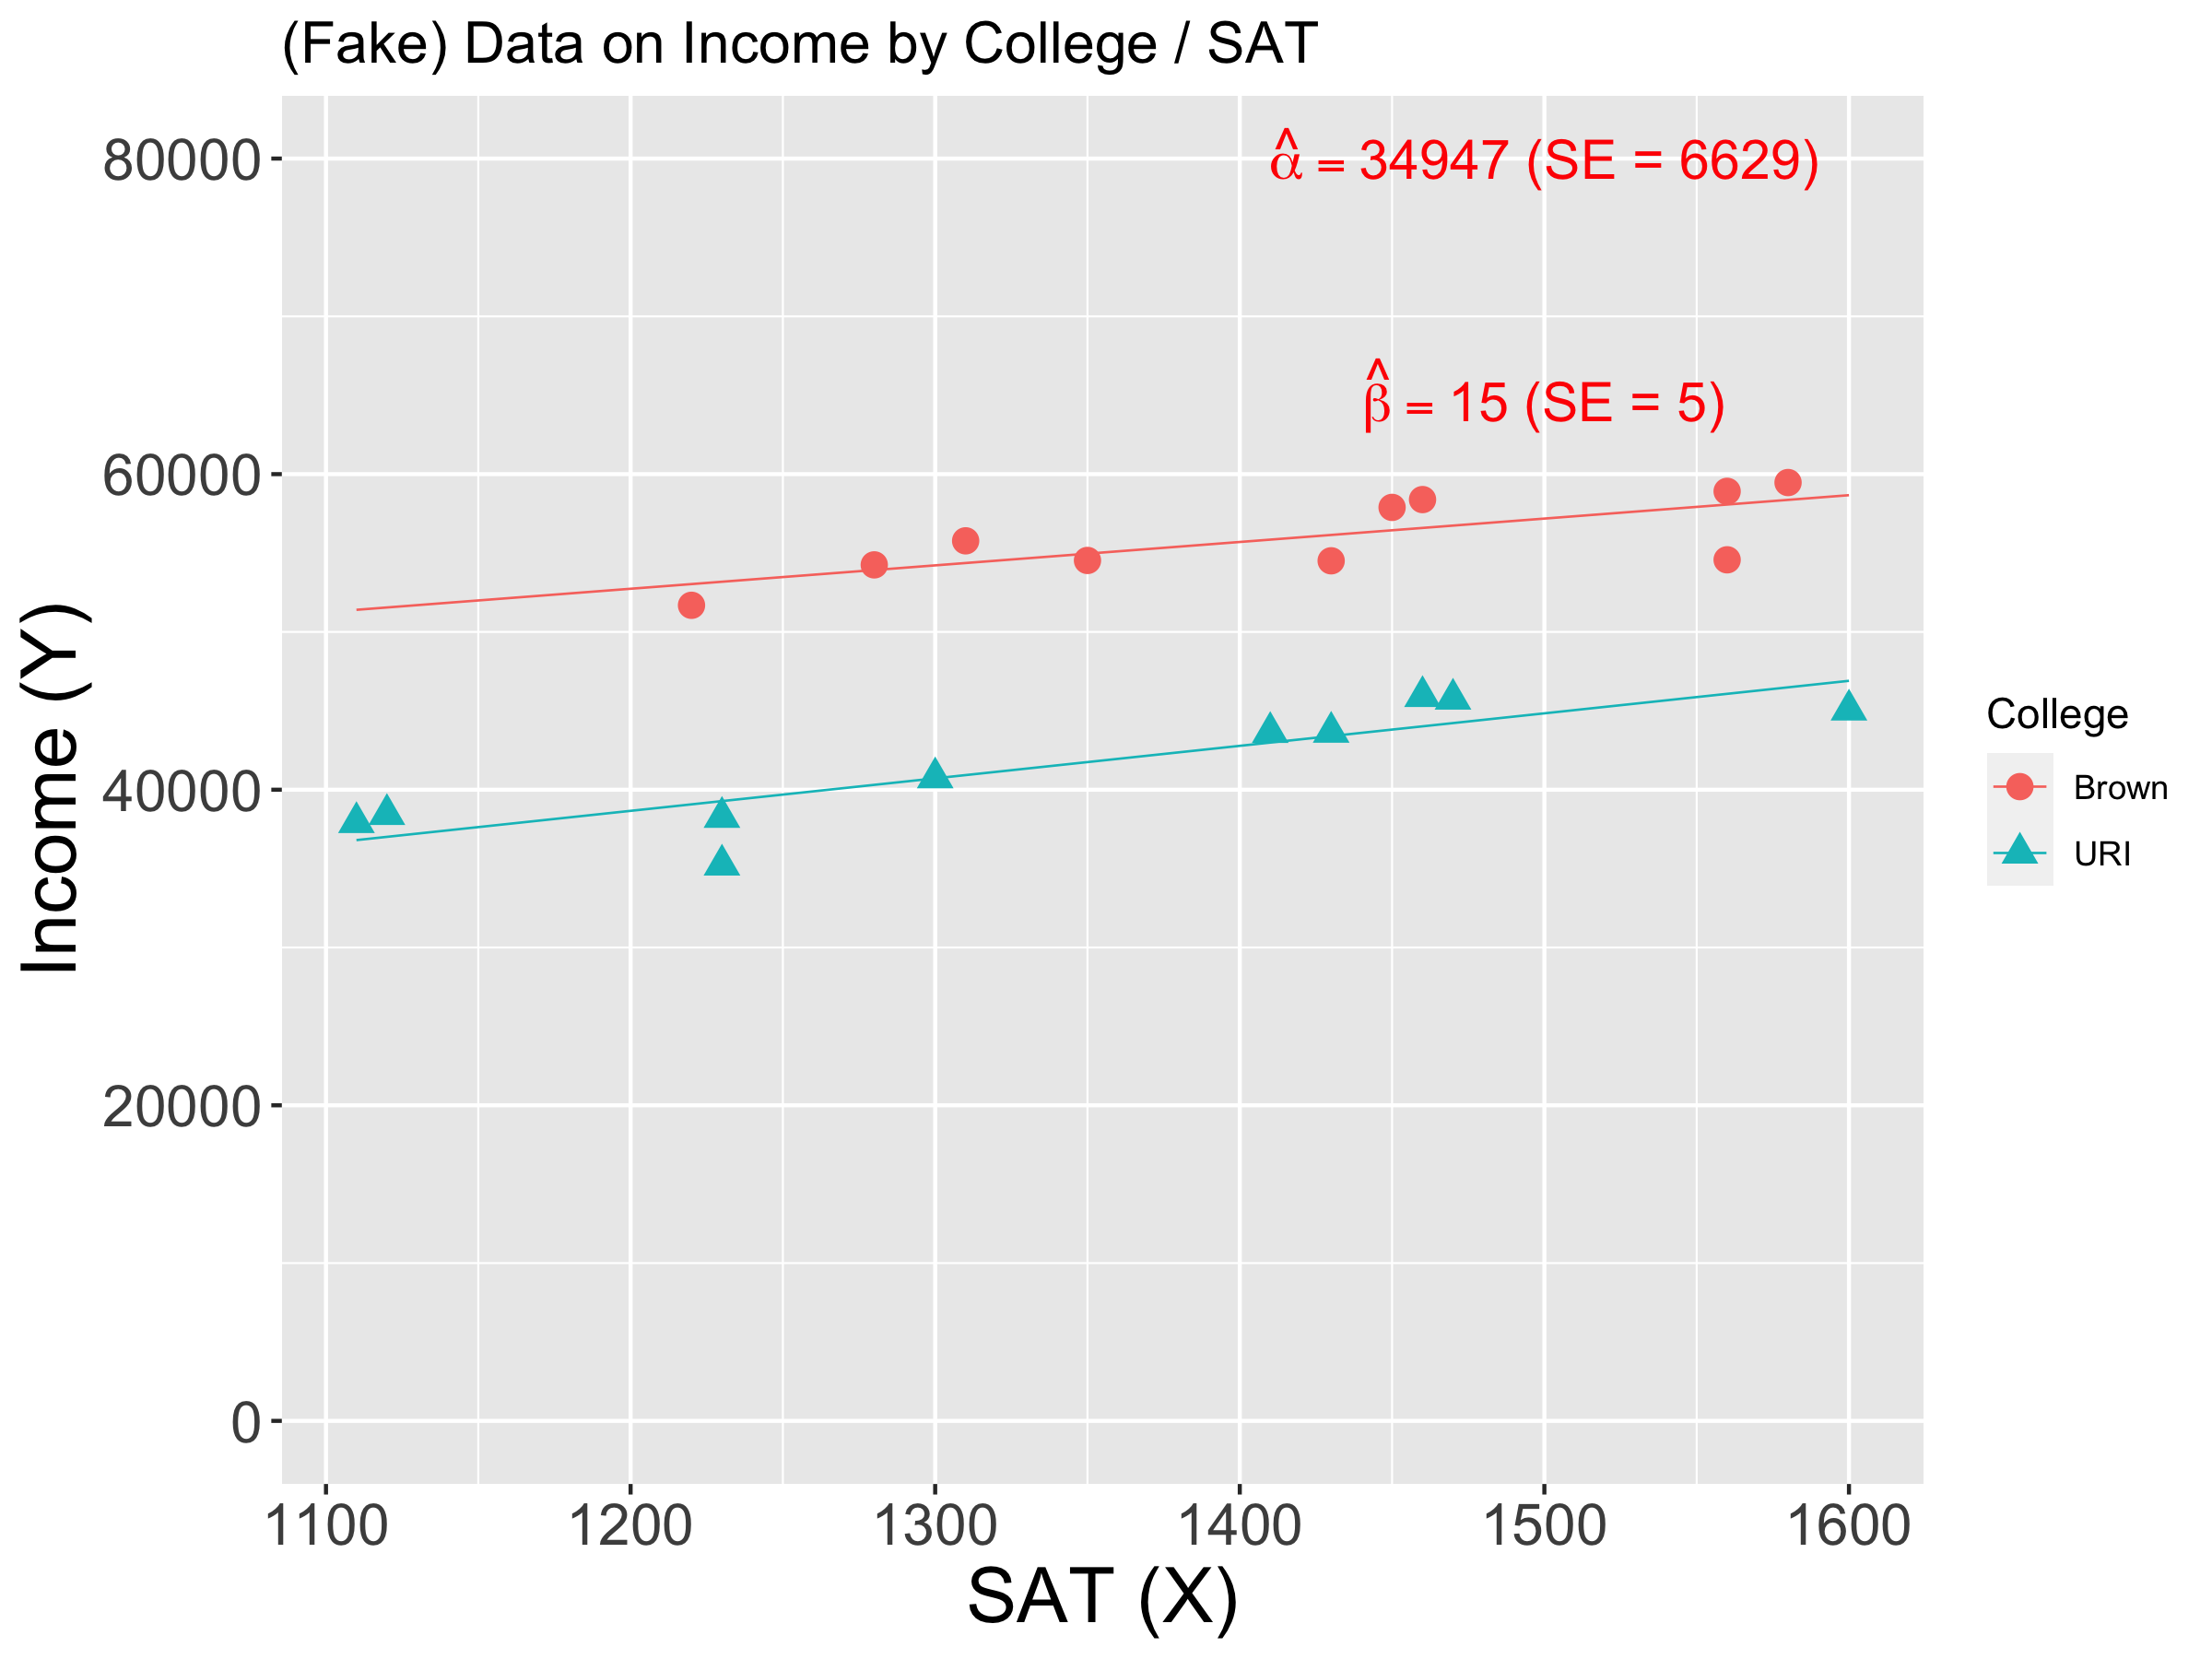
\includegraphics[scale=0.1]{fake-sat-with-trend-brown-betas-plus-ses.png}

\pause

\begin{wideitemize}
	\item
	Un CI para $\beta$ es  $\hat\beta \pm 1.96 \times SE \pause{} \approx [5,25]$
\end{wideitemize}
\end{frame}		
		

\begin{frame}{Regression como aproximación al CEF}
	\begin{wideitemize}
	\item
	Hasta ahora asumimos que el CEF es lineal: $E[Y_i | X_i = x]  = \alpha + \beta x$
	
	\item
¡¿Qué pasa si no lo es?!
	
	\pause
	\item
	Claim: si CEF no es lineal, entonces OLS nos da la ``mejor aproximación lineal'' que hay
	\pause 
	\item
	 Con eso me refiero a que $\alpha,\beta$ de OLS minimiza
	 
	 $$min_{\alpha,\beta} E[ (E[Y|X]  - (\alpha + \beta X) )^2 ]$$
	 
	 \pause
	 Es decir,  tenemos la función lineal  ``más cercana'' al CEF en términos de error cuadrático medio
	\end{wideitemize}
\end{frame}


\begin{frame}
		
	\begin{center}
		\hspace{0.7cm}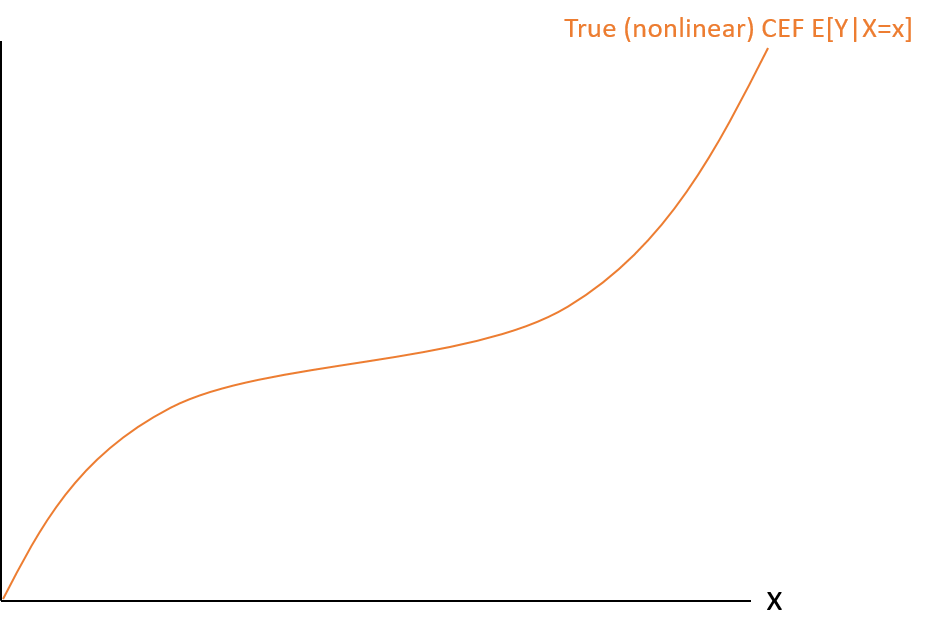
\includegraphics[scale=0.7]{ols1.png}
	\end{center}
	
\end{frame}

\begin{frame}
	
	\begin{center}
		\hspace{0.7cm}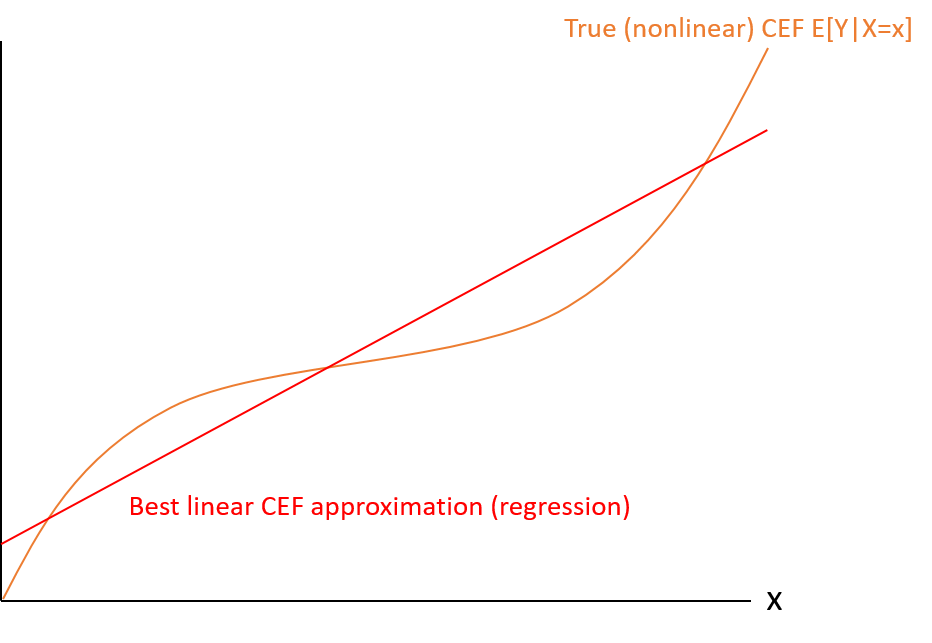
\includegraphics[scale=0.7]{ols2.png}
	\end{center}
	
\end{frame}

\begin{frame}
	
	\begin{center}
		\hspace{0.7cm}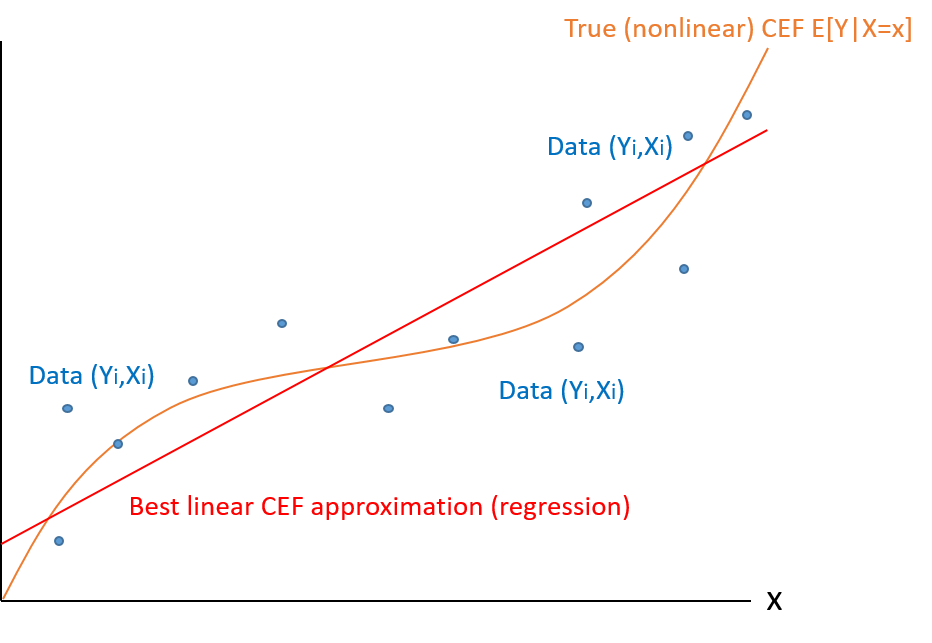
\includegraphics[scale=0.7]{ols3.png}
	\end{center}
	
\end{frame}

\begin{frame}
	
	\begin{center}
		\hspace{0.7cm}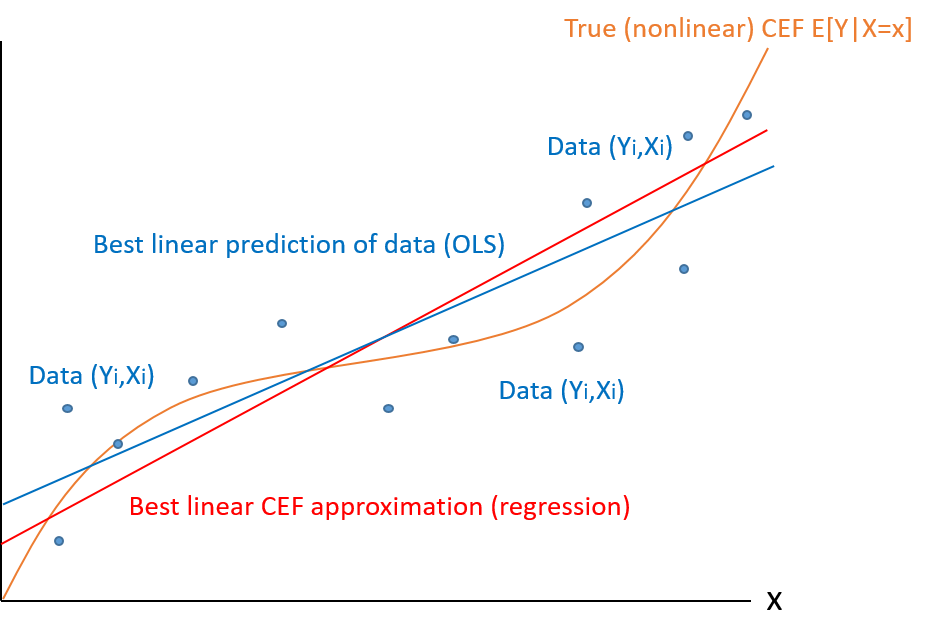
\includegraphics[scale=0.7]{ols4.png}
	\end{center}
	
\end{frame}

%%%%%%%%%%%%%%%%%% Clase Parte II 
\begin{frame}
\begin{center}
{\Huge \textbf{Fin de la parte I}}
\end{center}
\end{frame}

\begin{frame}{La clase pasada\dots}
La clase pasada vimos como podemos aproximar la función de esperanza condicional (en variables que observamos $X_i$) en una forma lineal 
\begin{align*}
E[Y_i \mid X_i =x ] \approx \alpha + x \beta ,
\end{align*}
cuando $X_i$ es un escalar (es decir, $X_i\in \mathbb{R}$ en lugar de ser un vector en $\mathbb{R}^k$).
			\begin{itemize}
					\item 
					Y mostramos como el estimando ($\alpha$,$\beta$) se puede estimar por OLS
				\end{itemize}

\vspace{.5cm}
Esto se puede generalizar al caso donde observas varias características $X_{i1}, X_{i2}, \dots, X_{ik}$. Simplemente podemos escribirlo en forma de vectores. 
\begin{align*}
E[Y_i| \mathbf{X}_i =\mathbf{x} ] \approx \mathbf{x}' \bm{\beta} \text{ dado un vector } \mathbf{X_i} = (1,X_{i1},...,X_{iK})'
\end{align*}

\end{frame}

	
	\begin{frame}{Plan para hoy}

	1. Introducción a Machine Learning
	\vspace{0.8cm}
	
	2. Comandos de Stata para ML
	
	\end{frame}
	
	
\end{document}


